\documentclass[a4paper,12pt]{report}
\usepackage[utf8]{inputenc}
\usepackage[english]{babel}
\usepackage{amssymb}
\usepackage{amsmath}
\usepackage{amsthm}
\usepackage{mathrsfs}
\usepackage[nottoc]{tocbibind}
\usepackage[backend=biber,style=alphabetic]{biblatex}
\usepackage{graphicx}
\usepackage[left=3cm, right=3cm, top=3cm, bottom=3cm]{geometry}
\usepackage{listings}
\usepackage{algpseudocode}
\usepackage[bookmarks=true,hidelinks]{hyperref}
\usepackage{color}
\usepackage{subfigure}
\usepackage{multirow}
\usepackage{enumitem}

\newtheorem{algorithm}{Algorithm}
\newtheorem{definition}{Definition}

\setcounter{secnumdepth}{3} % include subsubsection in section numbering
\setcounter{tocdepth}{3} % include subsubsection in toc

\setitemize{itemsep=1pt} % reduce vertical spacing

%% Create python environment
%% http://tex.stackexchange.com/questions/199375/problem-with-listings-package-for-python-syntax-coloring

% Defining colors
\definecolor{deepblue}{rgb}{0,0,0.5}
\definecolor{deepred}{rgb}{0.6,0,0}
\definecolor{deepgreen}{rgb}{0,0.5,0}

\newcommand\pythonstyle{\lstset{
  language=Python,
  backgroundcolor=\color{white}, %%%%%%%
  basicstyle=\footnotesize\ttfamily,
  otherkeywords={self,def,for,@property},            
  keywordstyle=\bf\color{deepblue},
  emph={Segmenter,ColorClassifier,PolygonClassifier,SquareRule,CircleRule,DispatchingRule,CustomSegmenter,WorkflowBuilder,NumpyImage,__init__},          
  emphstyle=\bf\color{deepred},    
  stringstyle=\color{deepgreen},
  commentstyle=\color{red},  %%%%%%%%            
  showstringspaces=false            
}}

% Python environment
\lstnewenvironment{python}[1][]
{
\pythonstyle
\lstset{#1}
}
{}

%% To uncomment if needed
%\usepackage{array}
%\usepackage[usenames,dvipsnames]{color}
%\usepackage{arydshln}
%\usepackage{slashbox}
%\usepackage{pdflscape}
%\usepackage{cancel}
%\setlist[itemize,1]{label=$\bullet$}

%% Add bibliography database
\addbibresource{bibliography.bib}

%% Set document data
\author{Mormont Romain}
\title{A workflow for computer-aided cytology and its applications}
\date{Academic year 2015-2016}

\begin{document}
	
	% Start frontpage =========================
	\thispagestyle{empty}
{ \sf

\begin{center}
	{\small University of Liège}\\
	{\small Faculty of Engineering}
\end{center}

\vfill

% Logo 
\begin{figure}[!h]
	\center
	
\includegraphics[scale=0.2]{image/institution_ulg.png}
\end{figure}

\vfill

\begin{center}
	{\LARGE Master Thesis\\}
\end{center}

\noindent\rule{1\linewidth}{1px}

\begin{center}
	{\LARGE \sf \textbf{A workflow for large-scale computer-aided cytology and its applications}.}
\end{center}

\noindent\rule{1\linewidth}{1px}

\begin{center}
	\textit{Author} : Romain Mormont
\end{center}

\begin{center}
	\textit{Supervisor} : Dr. Raphaël Marée
\end{center}

\begin{center}
	\textit{Academic} : Prof. Pierre Geurts
\end{center}
\vfill

\begin{center}
	Master thesis submitted for the degree of \\
	\vspace{0.25cm}
	{\Large MSc in Computer Science and Engineering}
\end{center}

\vfill
\begin{center}
Academic year 2015-2016\\
\end{center}
}
	% End frontpage ===========================
	
	\newpage 
	\clearpage
	\pagenumbering{gobble}
	
	% Start summary ===========================
	\section*{Abstract}
	\begin{center}
 
	{\sf \large \textbf{A workflow for large-scale computer-aided cytology and its applications}.}\\
\raggedleft
 	{\sf \textit{by Romain Mormont} }\\
\centering
	{\sf \textit{Supervisor}: Dr. Raphaël Marée, \textit{Academic}: Prof. Pierre Geurts }\\
\centering
	{\sf Academic year 2015-2016 }\

\end{center}
\hfill

In several fields of application, multi-gigapixel images must be analysed to gather information and take decision. This analysis is often performed manually, which is a tedious task given the volume of data to process. For instance, in cytology, branch of medical sciences which focuses on study of cells, cytopathologists analyse cell samples microscope slides in order to diagnose diseases such as cancers. Typically, malignancy is assessed by the presence or absence of cells with given characteristics. In geology, climate variations can be analysed by studying the concentration 
of micro-organisms in core samples. The concentration is usually evaluated by smearing the samples onto microscope glass slides and counting those micro-organisms. \\

In those situations, computer sciences and, especially, machine learning and image processing provide a great alternative to a pure-human approach as they can be used to extract relevant information automatically. Especially, those kind of problems can be expressed as object detection and classification problems.
\\

This thesis presents the elaboration and assessment of a generic framework, \textit{SLDC}, for object detection and classification in multi-gigapixel images. Especially, this framework provides implementers with a concise way of formulating problem dependent-components of their algorithm (i.e. segmentation and classification) while it takes care of problem-independent concerns such as parallelization and large image handling. 
\\

The performances of the framework are then assessed on a real-world problem, thyroid nodule malignancy. Especially, a workflow is built to detect malignant cells in thyroid cell samples whole-slides.
\\

Results are promising: the effective processing time for an image containing 8 gigapixels is less than 10 minutes. In order, to further reduce this execution time, some improvements are proposed.
\\

The framework implementation can be found on GitHub: \url{https://github.com/waliens/sldc}.

\hfill
	\newpage
	% End summary =============================
		
	% Start acknowledgement ===================
	\section*{Acknowledgement}
	First, I would like to thank Raphaël Marée for the time he dedicated to guide and advise me throughout the making of this thesis. His support has been a great help which has undoubtedly contributed to the final result. 
\\

Then, I would like to thank Pierre Geurts for his guidance and, especially, for his advices regarding the redaction of this manuscript. I am also grateful to him for introducing me to Raphaël Marée and therefore allowing me to work on such an interesting subject. 
\\

I would also like to thank Renaud Hoyoux for his availability and quickness at solving bugs which sometimes prevented be from getting further.
\\

A great thank to Jean-Michel Begon for his availability to answer my question about his implementation. 
\\

Finally, I would like to address my gratitude to my friends and family for their support. Especially, I address a special thank to Floriane, Justine and Fabrice who have accepted to proofread this manuscript.



	\newpage
	% End acknowledgement =====================
	
	% Start table of content ==================
	\tableofcontents
	% End table of content ====================
	
	\newpage
	\clearpage
	\pagenumbering{arabic}
	
	% Start introduction ======================
	\chapter{Introduction}
	In several domains, multi-gigapixel images must be analysed for the purpose of gathering information and/or for taking decisions. Typically, the information is represented by the presence of a series of objects of interest which are embedded into the image. The aim of the analysis is to locate and identify those objects. Depending on the problem and  specific field of application, the extracted objects can be used for various purposes. For instance, in cytology, digitized microscope slides containing human tissues are analysed by physicians in order to diagnose particular diseases, the disease in question manifesting itself by the presence of cells having certain characteristics. In geology, slides containing core samples can be digitized and analysed to find concentration of certain micro-organisms.

Those images are usually analysed manually by experts. However, due to the size of the problem, the analysis is not always performed exhaustively. When possible, experts typically select a reduced number of regions to study and draw conclusions from the observations performed in those regions. This process has obviously the drawback of increasing the risk of missing objects of interest.

Because of the risk yielded by the previous method and because manual analysis of full images is long and tedious, computer programs could be used to assist experts. For instance, those programs could indicate which regions are worth analysing and which are not. They could also perform the search instead of the expert but under his supervision: that is, the expert would be able to provide a feedback to the program which could then improve its detection process. 

In order to provide this assistance and to learn from experts' feedbacks, image processing and machine learning are used. Whereas IP and ML provide a complete toolbox of algorithms for computer vision in general, they are however not necessarily well suited for handling large images. Especially, typical implementations of those algorithms implicitly make the assumption that the full image can be loaded into memory which is not always possible. Indeed, multi-gigapixel images typically require several gigabytes of memory. As far as the execution times of those algorithms are concerned, they generally grow with the size of the image, yielding unacceptable execution times. Parallelism can alleviate this problem but, again, typical implementations do not necessarily support this feature. Therefore, when diving into a new problem of object detection, implementers typically develop workflows by combining machine learning and image processing algorithms to handle detection but they also have to deal with problem-independent concerns such as parallelism or memory constraints. 

This thesis proposes \textit{SLDC}, a generic framework for solving problems of object detection and classification in multi-gigapixel images. Especially, it provides implementers with a structure to define problem-dependent components of the algorithm (i.e. detection and classification) in a concise way. Every other concerns such as parallelization and large image handling are encapsulated by the framework. The framework also provides a way to execute several processing workflows one after another on the same image as well as a powerful and customizable logging system. 

In Chapter \ref{chap:context}, the problem of object detection and classification is introduced and its application to different cases is presented. In Chapter \ref{chap:work_intro}, the framework and its implementation are presented. In Chapter \ref{chap:thyroid}, the framework is applied to a cytology problem, the thyroid case.
	\newpage
	% End introduction ========================
	
	% Start chapter 1 : obj. detection ========
	\chapter{Object detection in multi-gigapixel images and applications}
	\section{General problem}
\subsection{Formulation}
Generic formulation of the object detection problem
\subsection{Implementation issues}
What issues an implementor could face when trying to implement object detection in large images
\subsection{Related works}
What solutions are usually presented in the litterature to solve those problems (shallow overview as this is a wide topic) 
\section{Cytology}
\subsection{An object detection problem ?}
Why it is an instance of the "object detection in large images" problem
\subsection{The thyroid case}
Explanation of the Thyroid case 
	\newpage
	% End chapter 1 : obj. detection ==========	
	
	% Start chapter 2 : generic workflow ======
	\chapter{A generic workflow : Segment Locate Dispatch Classify}
	In this chapter, a generic workflow for solving problems of objects detection and classification in images is presented. The history of this workflow is presented in Section \ref{sec:history_first_dev}. Section \ref{sec:workflow_principle} introduces the workflow itself. Finally, the implementation carried out in the context of this thesis is presented and discussed in Section \ref{sec:workflow_impl}.

\section{History and first developments}
\label{sec:history_first_dev}
The Segment-Locate-Dispatch-Classify (SLDC) workflow was first imagined by ?? Jean-Michel Begon ?? as a generalization of the work on thyroid nodule malignancy detection made in \cite{adeblire2013}. In the context of his master thesis, the author had implemented a processing workflow for detecting cells with inclusion and proliferative architectural patterns (see ?? (thyroid)) in digitized thyroid punctions slides. The cells and architectural patterns were detected by segmenting the images and then classified using machine learning techniques. As explained in the Section ?? (thyroid), some patterns could themselves contain cells with inclusion. Therefore, the author implemented a second processing workflow to detect those cells. This workflow was similar to the first because it relied on a segmentation algorithm to isolate cells in patterns and then used machine learning to assess their malignity. 

From those workflows, a common pattern emerged: performing detection using a segmentation algorithm and then classifying the detected objects using machine learning techniques. In 2015, ?? Jean-Michel Begon ?? developed a first version of a generic workflow based on this pattern and gave it the name \textit{Segment-Locate-Dispatch-Classify}. Then, he applied its workflow to the thyroid case. Unfortunately, this implementation suffered from some drawbacks which made it hard to reuse in other contexts. The workflow was therefore re-worked in the context of this master thesis.

\section{Principle}
\label{sec:workflow_principle}

\subsection{Algorithm}
\label{ssec:workflow_algo}
The workflow is a meta-algorithm\footnote{In this context, a meta-algorithm is an algorithm that coordinates the execution of other algorithms.} that detects and classifies objects contained in images. Particularly, given a two-dimensional\footnote{A third dimension can be dedicated to the images channel (i.e. 3 channels for RGB images, 4 channels for RGBA images).} image $\mathcal{I}$ as input, it is expected to output the information about the objects of interest in this image. Those information include the shape of the object, its location in the image as well as a classification label. Formally, the workflow can be seen as an operator $\mathcal{W}$:

\begin{definition} Let $\mathcal{W}$ be an operator such that 
	\begin{equation}\label{eqn:workflow_operator}
		\mathcal{W}(\cdot) : \mathcal{I} \rightarrow \left\{(o_1,C_1),...,(o_N, C_N)\right\}
	\end{equation}
	where $N$ is the number of objects of interest in $\mathcal{I}$ and $(o_i, C_i)$ is a tuple. The first element of this tuple, $o_i$, is a representation of the information (shape and location) about the $i^{th}$ object of interest found in $\mathcal{I}$ and the second, $C_i$, its classification label. 
\end{definition}

It is worth noting that genericity is of the essence. That is, the meta-algorithm should be able to solve the widest possible range of object detection and classification problems. Moreover, as explained in Section \ref{sec:history_first_dev}, it should produce those outputs using image segmentation and machine learning. As far as the segmentation is concerned, genericity is usually hard to obtain because of the high variability of images across different problems. In order to ensure genericity, the workflow doesn't impose a particular segmentation procedure but expects the implementer to provide one that suits the problem. The same goes for the classification models used for predicting the labels of the objects. 

In the subsequent sections, some additional operators are defined and used to build the $\mathcal{W}$ operator. First, a basic version of the algorithm is presented and then refined in order to achieve an acceptable level of genericity.

\subsection{Additional operators}
\label{ssec:other_operators}

Segmentation is the first operation applied to the image. This step of the algorithm is where the detection is actually carried out:
 
\begin{definition} \label{def:segmentation_op}
Let $\mathcal{S}$ be the \textbf{segment} operator. It is applied to an image $\mathcal{I}$ and produces a binary mask $\mathcal{B}$. The pixel $b_{ij}$ of $\mathcal{B}$ is 1 if the pixel $p_{ij}$ of $\mathcal{I}$ is located in an object of interest, otherwise it is 0. Formally:
\begin{equation}
	\label{eqn:operator_segment}
	\mathcal{S}(\cdot) : \mathcal{I} \rightarrow \mathcal{B}
\end{equation}
\end{definition}

While the segmented image theoretically contains the necessary information about the detected objects (i.e. shape and position in the image), the format of this information is inconvenient to query mostly because it is embedded into the binary mask and a single object cannot be trivially extracted. An intermediate step that would convert this information into a more convenient format is therefore needed. This format should encode both the shape of the object and its position in the image. It appears that polygons match this specification. 

\begin{definition} \label{def:locate_op}
Let $\mathcal{L}$ be the \textbf{location} operator. It is applied to a binary mask and produces a set of polygons encoding the shapes and positions of every object in the image. Formally:

\begin{equation}
	\mathcal{L}(\cdot) : \mathcal{B} \rightarrow \left\{P_1, ..., P_N\right\}
\end{equation}

where $\mathcal{B}$ is a binary mask as defined in Definition \ref{def:segmentation_op}, $N$ is the number of objects of interest in $\mathcal{B}$ and $P_i$ is the polygon representing the geometric contour of the $i^{th}$ object in $\mathcal{B}$.
\end{definition}

The final step of the workflow is the object classification and is performed by a classifier which is passed a representation of the object (e.g. image, geometric information,...) and produces a classification label. In this theory, there is no restriction about the nature or representation of the objects processed by the classifiers.

\begin{definition} Let $\mathcal{T}$ be the \textbf{classifier} operator. It is applied to an object of interest and produces a classification label. Formally:
\begin{equation}
	\mathcal{T}(\cdot) : o \rightarrow C
\end{equation}
where $o$ is the object and $C$, the classification label. 
\end{definition}
\begin{definition}
Let $\mathcal{T}^*$ be an extension of $\mathcal{T}$ which is given a set of objects and produces labels for all of them. Formally: 
\begin{equation}
	\mathcal{T}^*(\cdot) : \left\{o_1, ..., o_N\right\}  \rightarrow \left\{C_1, ..., C_N\right\}
\end{equation}
\end{definition}

\subsection{Single segmentation, single classifier}
\label{ssec:single_single}

The most simple construction of $\mathcal{W}$ would be the composition of the operators defined in Section \ref{ssec:other_operators}. Particularly, the compositions $\mathcal{S} \circ \mathcal{L}$ and $\mathcal{S} \circ \mathcal{L} \circ \mathcal{T}^*$ would respectively produce the polygons representing the objects and and their labels. This construction is summarized in Algorithm \ref{algo:single_seg_single_classif}: 

\begin{algorithm} \label{algo:single_seg_single_classif} 
	Construction of $\mathcal{W}$ using one segmentation and one classifier:
	
	\begin{enumerate}
		\item Return $\left(\mathcal{S} \circ \mathcal{L}\right)\left(\mathcal{I}\right) \times \left(\mathcal{S} \circ \mathcal{L} \circ \mathcal{T}^*\right)\left(\mathcal{I}\right)$
	\end{enumerate}
\end{algorithm}

As explained in Section \ref{ssec:workflow_algo}, the definition of $\mathcal{S}$ and $\mathcal{T}^*$ would be left at the implementer's hands. As far as the $\mathcal{L}$ operator is concerned, it could be imposed by the workflow without loss of genericity. Such an construction of $\mathcal{W}$ could already solve any object detection and classification problem on image in which the labels can be predicted by a single classifier. However, in some cases, one classifier is not enough. This happen, for instance, when the image contains objects of very different nature and using several classifiers would yield better results than using a single one. An extension is therefore needed.

\subsection{Single segmentation, several classifiers}
\label{ssec:single_several}

In this attempt to construct a generic $\mathcal{W}$ operator, the image is assumed to contain $M$ distinct types of objects and the workflow uses $M$ classifiers (the $i^{th}$ classifier being noted as $\mathcal{T}_i$ with $i \in \{1,...,M\}$) to classify those objects. As an object should only be processed by one classifier, the workflow has to be added a new step which consists in dispatching each polygon to its most appropriate classifier. 

\begin{definition}\label{def:dispatch_op} 
	Let $\mathcal{D}$ be the dispatch operator. It is applied to a polygon and produces an integer which identifies the most appropriate classifier for processing this polygon: 

	\begin{equation}
		\mathcal{D}(\cdot) : P \rightarrow i, i \in \{1,...,M\}
	\end{equation}
\end{definition}

This step being problem dependent, it is the responsibility of the implementer to define the rules used for dispatching the polygons. However, the format of these rules can be defined.

\begin{definition} 
	Let $\mathcal{P}$ be a set of $M$ predicates $p_1, ..., p_M$ which associate truth values to polygons:
	\begin{equation}
		p_i(\cdot) : P \rightarrow t \in \{true, false\}, i \in \left\{1,...,M\right\} 
	\end{equation}
	where $p_i$ is the predicate associated with the $i^{th}$ classifier. The polygon $P$ is dispatched to a classifier $\mathcal{T}_i$ if $p_i$ associates true to this polygon. To avoid dispatching an object to several classifier, the predicates should verify the following property:
	\begin{equation}
		p_i = true \Leftrightarrow p_j = false, \forall j \neq i
	\end{equation} 
\end{definition}

Given this format, the $\mathcal{D}$ operator can be trivially constructed as it returns $i$ if $p_i$ is \textit{true}. The algorithm resulting from this construction of $\mathcal{W}$ starts the same way as in Section \ref{ssec:single_single}: the image is applied the segment and locate operators. Then, the resulting polygons are dispatched and classified to produce the classification label. The resulting algorithm is summarized in Algorithm \ref{algo:single_seg_several_classif}. 

While the range of problems that can be solved using this algorithm has been increased compared to the version with a single classifier, there are still some problems that cannot be. In particular, if some objects are included into other bigger objects, they won't be considered as independent objects. 

Before extending the algorithm for handling this case, it is worth noting that Algorithm \ref{algo:single_seg_several_classif} is completely compatible with Algorithm \ref{algo:single_seg_single_classif}. Indeed, if there is only one classifier (i.e. $M = 1$) and the predicate $p_1$ always returns $true$, then both algorithms are exactly the same. 

\begin{algorithm}\label{algo:single_seg_several_classif}
Construction of the $\mathcal{W}$ operator with a single segmentation and several classifiers. 
\begin{enumerate}
	\item Apply the $\mathcal{S} \circ \mathcal{L}$ composition to the input image $\mathcal{I}$ to extract the objects of interest as the set of polygons $S_p \leftarrow \left\{P_1, ..., P_N \right\}$
	\item Initialize the labels set $L \leftarrow \emptyset$
	\item For each polygon $P \in S_p$:
	\begin{enumerate}
		\item Compute the classification label $C \leftarrow \mathcal{T}_{\mathcal{D}(P)}(P)$
		\item Place the label in the labels set $L \leftarrow L \cup \{C\}$
	\end{enumerate}
	\item Build and return objects and labels set $S_p \times L$.
\end{enumerate}
\end{algorithm}

\subsection{Chaining workflows}

To handle the case when objects of interest can be included into objects of bigger size in the image, a solution consists in executing several instances of Algorithm \ref{algo:single_seg_several_classif} sequentially one after another. 

\begin{definition}\label{def:several_w_op}
	Let $\mathcal{W}_1, ..., \mathcal{W}_K$ be a set of $K$ instances of Algorithm \ref{algo:single_seg_several_classif}. Each algorithm $\mathcal{W}_i$ has its own segmentation procedure $\mathcal{S}_i$ and proper sets of dispatching predicates $\mathcal{P}_i$ and classifiers $S_{\mathcal{T},i}$.
\end{definition}

While $\mathcal{W}_1$ would be applied to the full image $\mathcal{I}$ to extract all the objects of interest, $\mathcal{W}_2, ..., \mathcal{W}_K$ are only passed image windows containing the previously detected objects.

\begin{definition}\label{def:image_window}
	Let $\mathcal{I}_P$ be an image window extracted from image $\mathcal{I}$ and containing the object represented by the polygon $P$. The window is the minimum bounding box containing this polygon.
\end{definition}

A further refinement would be to provide a way for the implementer to filter the polygons of which the windows are passed to a given workflow instance. Indeed, a given instance $\mathcal{W}_i$ might be designed to process only a certain category of objects and therefore should not be passed windows of objects that doesn't fall in this category. 

\begin{definition}\label{def:filter_op}
	Let $\mathcal{F}$ be the $\textbf{filter}$ operator. It is given a set of polygons $S_P$ and returns a subset $S'_P$ of polygons:
	
	\begin{equation}
		\mathcal{F}(\cdot): S_P \rightarrow S'_P, S'_P \subseteq S_P
	\end{equation}
\end{definition}

Each instance of the workflow $\mathcal{W}_i$ except $\mathcal{W}_1$ is therefore associated a filter operator $\mathcal{F}_i$. The resulting algorithm is given in Algorithm \ref{algo:chaining_workflows} and has now reached an acceptable level of genericity.

\begin{algorithm} \label{algo:chaining_workflows}
	Construction of the $\mathcal{W}$ operator with $K$ instances of Algorithm \ref{algo:single_seg_several_classif}:

	\begin{enumerate}
		\item Execute the first workflow and save the results in the results set $R$: $R \leftarrow \mathcal{W}_1(\mathcal{I})$
		\item Create the polygons set and initializes it with the polygons found from the execution of $\mathcal{W}_1$: $S_P \leftarrow \left\{P_1, ..., P_N\right\}$
		\item For each $i \in \{2, ..., K\}$:
		\begin{enumerate}
			\item Extract polygons to be processed by $\mathcal{W}_i$: $S'_P \leftarrow \mathcal{F}_i(S_P)$
			\item For polygon $P \in S'_P$:
			\begin{enumerate}
				\item Execute workflow $\mathcal{W}_i$ on the image window and saves the results: $R \leftarrow R \cup \mathcal{W}_i(\mathcal{I}_P)$
				\item Add the extracted polygons to the polygons set: $S_P \leftarrow S_P \cup \left\{P_1, ..., P_M\right\}$
			\end{enumerate}
		\end{enumerate}
		\item Return the results set $R$
	\end{enumerate}
\end{algorithm}

\section{Implementation}
\label{sec:workflow_impl}
The workflow presented in Section \ref{sec:workflow_principle} is now defined. This section details the design choices and architecture of the implementation. In the subsequent sections, the term workflow will refer to the algorithm while the term framework will refer to the implementation.

\subsection{Requirements}
The main requirements for the framework are listed hereafter.

\paragraph{Genericity} As for the algorithm, the framework should be able to solve the widest possible range of objects detection and classification problems in any context. This property has more implication in the case of the framework design than for the algorithm design, especially when it comes to fixing the representation of the various involved data types (i.e. image, polygon,...). Moreover, the implementer should be able to do whatever he wants to do with the results of the computations. 

\paragraph{Efficiency} While the framework has no control over the efficiency of the algorithms defined by the implementer (i.e. segmentation or classification procedures), the coordination of those algorithms should not induce a significant overhead in the overall execution. 

\paragraph{Large images} While large images handling was irrelevant at the algorithm design stage, it becomes critical at this point. To remain generic, the framework should not make any assumption about the size of the images to be processed. Especially, a whole image should not be assumed to fit into memory.

\paragraph{Robustness} The framework should be robust to errors. That is, a single error should not interrupt the whole execution. For instance, if the framework executes a set of independent computations and one of them fails, it should only be stopped if this failure is unrecoverable and affects all the other computations. Otherwise, the failure should be reported and those others computations should execute until completion. 

\paragraph{Transparency} The framework should provide a built-in way to communicate its progress as well as the errors it encounters with the user. The level of verbosity of this communication should be adjustable. 

\paragraph{Parallelism} Whenever possible the framework should take advantage of parallelism to reduce its execution time but the implementer should be able to switch from parallel execution to sequential execution and vice versa. Moreover, the implementer should be able to change the level of parallelism (i.e. the number of jobs available).

\paragraph{Ease of use} The work of the implementer should be kept as minimal as possible. He should only have to define the problem dependent elements of the workflow: segmentation, dispatching rules, classifiers,... 

\subsection{Language}
The first design choice occurring in the implementation of an existing algorithm is obviously the language in which this implementation will be made. As far as the workflow is concerned, the chosen language was Python. Indeed, this language provides a very complete environment for developing objects detection and segmentation algorithms which would obviously contribute to the overall ease of use the framework. What makes this environment complete ans some other reasons why Python was chosen are detailed hereafter.

First of all, Python has become a great language for scientific computing as it has been augmented with excellent open source libraries over the years. First, the SciPy ecosystem which includes the SciPy \cite{oliphant:2007} and NumPy \cite{vanderwalt:2011} libraries. The first is a collection of numerical algorithms and domain-specific toolboxes (signal processing, optimization, statistics,...). The second is a fundamental package for numerical computations which provides an efficient representation of multi-dimensional arrays and operations on them. Built on top of the SciPy ecosystem comes Scikit-Learn \cite{pedregosa:2011}, a library that provides simple, efficient and reusable tools for data mining and machine learning. Image processing is not outdone with a Python binding for the huge OpenCV library \cite{opencv_library}. Two alternatives are scikit-image \cite{scikit-image} which is built on top of the SciPy ecosystem or the Pillow library \cite{pillow}. All of them provide a collection of well-known image processing algorithms. Another useful library is Shapely \cite{shapely} which provides a representation for geometric objects such as polygons as well as operations to apply on them. 

Then, Python was also chosen because the workflow was implemented to be integrated with Cytomine (see Section ??). Particularly, the final goal was the detection and classification of objects in images stored on Cytomine servers. As those images and their metadata are exposed through an API interfaced by a Python client, it was essential that the workflow could use this client to communicate with the back-end. 

Finally, Python has many features which allows developers to quickly come up with solutions to problems. Especially, it is strongly and dynamically typed, multi-paradigm (imperative, functional, object oriented,...), interactive, interpreted and garbage-collected. 
 
\subsection{Software architecture}

\subsubsection{Image representation} 
The image representation manipulated by the framework is a critical point of the architecture. Indeed, on the one hand, it should be abstract enough so that implementers can apply the workflow to problems where they have their own image representation. On the other hand, it should provide access to a concrete representation that the steps of the workflow fixed by the framework (i.e. location) could use to extract necessary information. This is achieved by using two representations: an abstract one and a concrete one. As much as possible the framework works with the abstract representation and only switch to the other one when required. 

The representation should also provide a way of extracting sub-windows from an image. The application of this feature would be twofold. First, it is needed by the workflow (see Definition \ref{def:image_window}). Then, it could be used to address the large images handling requirement and to overcome the fact that a whole image is not assumed to fit into memory. Especially, the image would be splitted into smaller chunks called tiles and those tiles would be processed one after another.

The final design is shown in Figure \ref{fig:uml_image_package}.

Especially, the concrete representation is passed to the segmentation procedure (see operator $\mathcal{D}$ in Definiton \ref{def:segmentation_op}) and is also use to represent the binary mask produced by the segmentation and processed by the locate procedure (see $\mathcal{L}$ in \ref{def:locate_op}). 

\begin{figure}[h]
	\center 
	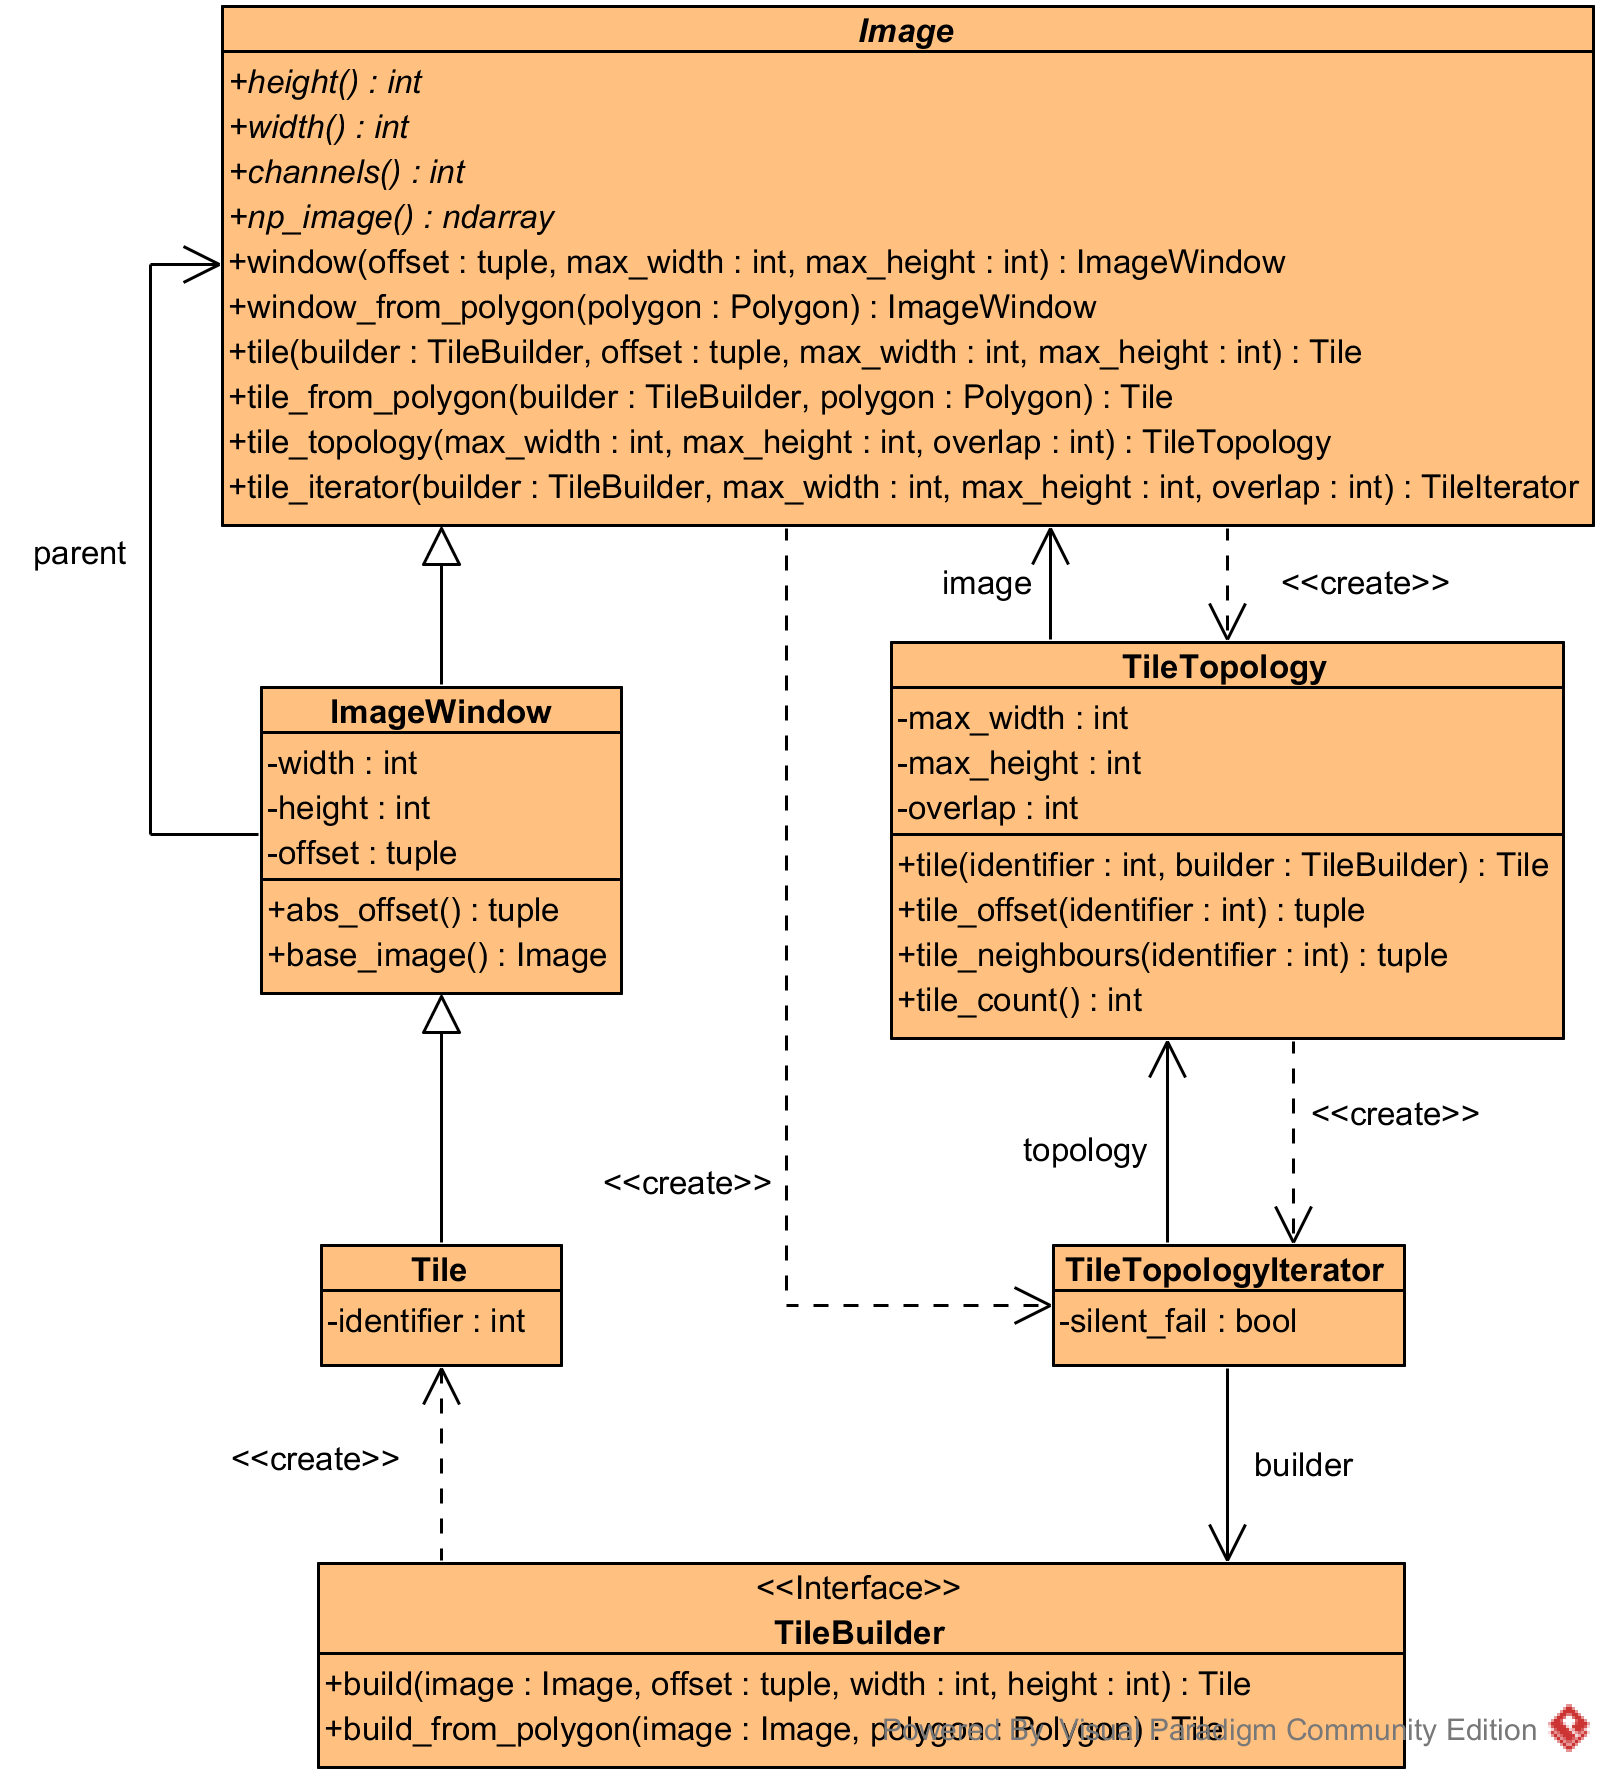
\includegraphics[scale=0.9]{image/uml_image_package.png}
	\caption{Image representation classes}
	\label{fig:uml_image_package}
\end{figure}

\subsection{How to use the framework}
A toy example: finding disks in an image with grey background and guessing whether they're black or white 
	\newpage
	% End chapter 2 : generic workflow ========
	
	% Start chapter 3 : thyroid case ==========
	\chapter{\textit{SLDC} at work : the thyroid case}
	In this chapter, the \textit{SLDC} framework is applied the problem presented in Chapter \ref{chap:context} : the nodule malignancy assessment. This problem is effectively an instance of the objects detection and classification problem. Indeed, the goal is to diagnose malignancy by the presence or absence of cells or groups of cells having particular characteristics in digitized microscope whole-slide. This problem is a good use case for the \textit{SLDC} framework: the images are large (i.e. typically 15 giga-pixels), two distinct categories of objects must be found (namely cells and groups of cells) and some of these objects can be included into others which can be handled using dispatching and chaining.  

An introduction to the thyroid problem as well as the underlying implementation challenges are presented in Section \ref{sec:thyroid_impl_issue}. Then, the workflow developed in \cite{adeblire2013} is briefly presented and its performances are assessed in Section \ref{sec:thyroid_adeblire_algo}. Especially, some flawed steps are highlighted and some improvements are proposed. Then, the implementation of the improved workfow is detailed in section \ref{sec:thyroid_implementation}. Finally, the performances of this implementation are analyzed in Section \ref{sec:thyroid_perf}.

\section{Problem and underlying challenges}
\label{sec:thyroid_impl_issue}
The problem consists in finding cells with inclusions and proliferative architectural patterns in large digitized microscope slides. To perform this detection, a dataset containing approximately 5700 annotations was created by experts on the Cytomine platform. The major challenges involved with this problem are detailed hereafter. 

\paragraph{Image quality} While the images resolution is more than acceptable, the images themselves are by nature not very well suited for object extraction. Indeed, the objects of interests are surrounded with a lot of other undesirable objects. Moreover, due to the imprecise nature of the staining performed before digitization, some staining variations appears from one slide to another but also within a single slide. 

\paragraph{Image size} As explained in Section \ref{sssec:detection_thyroid_dataset}, the size of the images ranges from 4 giga-pixels to 18 giga-pixels. Therefore, the various processing steps should be as efficient as possible to avoid huge execution times. Also, accessing the images must be done through HTTP requests. Therefore, a particular attention should be paid to the number of requests to be executed for fetching the image. Especially, some caching policy might be needed to reduce the network time overhead. 

\paragraph{Class imbalance} The dataset of annotations is relatively balanced if all terms are considered separately. However, grouping terms for expressing the detection as a binary (or ternary) problem results in a major class imbalance, especially for the cells with inclusion versus normal cells problem. 

\paragraph{Human annotations} The human annotations are imperfect as experts usually annotate objects roughly (i.e. an annotation can be larger than the actual object). Moreover, some annotation drawing tools provided on the Cytomine platform generate particular shapes such as circles or rectangles. Assuming that an algorithm will annotate the cells more precisely, the resulting  differences in terms of geometry and information content of the crops might lead to poor results if the experts annotations are used as learning data. 


\section{First workflow}
\label{sec:thyroid_adeblire_algo}

The workflow developed by Antoine Deblire in \cite{adeblire2013} is summarized in Figure \ref{fig:workflow_adeblire}. The idea behind this workflow is fairly simple. A first segmentation is applied to extract standalone cells and architectural patterns (step 4.3). The detected objects are then differentiated using their area and circularity (step 4.4) and dispatched to a classifier (steps 4.6). Especially, architectural patterns are classified as proliferative or non-proliferative by a first classifier and the cells are classified as inclusion or normal by a second one. Then, architectural patterns are segmented again (step 4.5) to extract the cells they contain and those cells are also passed to the cell classifier. 

\begin{figure}
	\center
	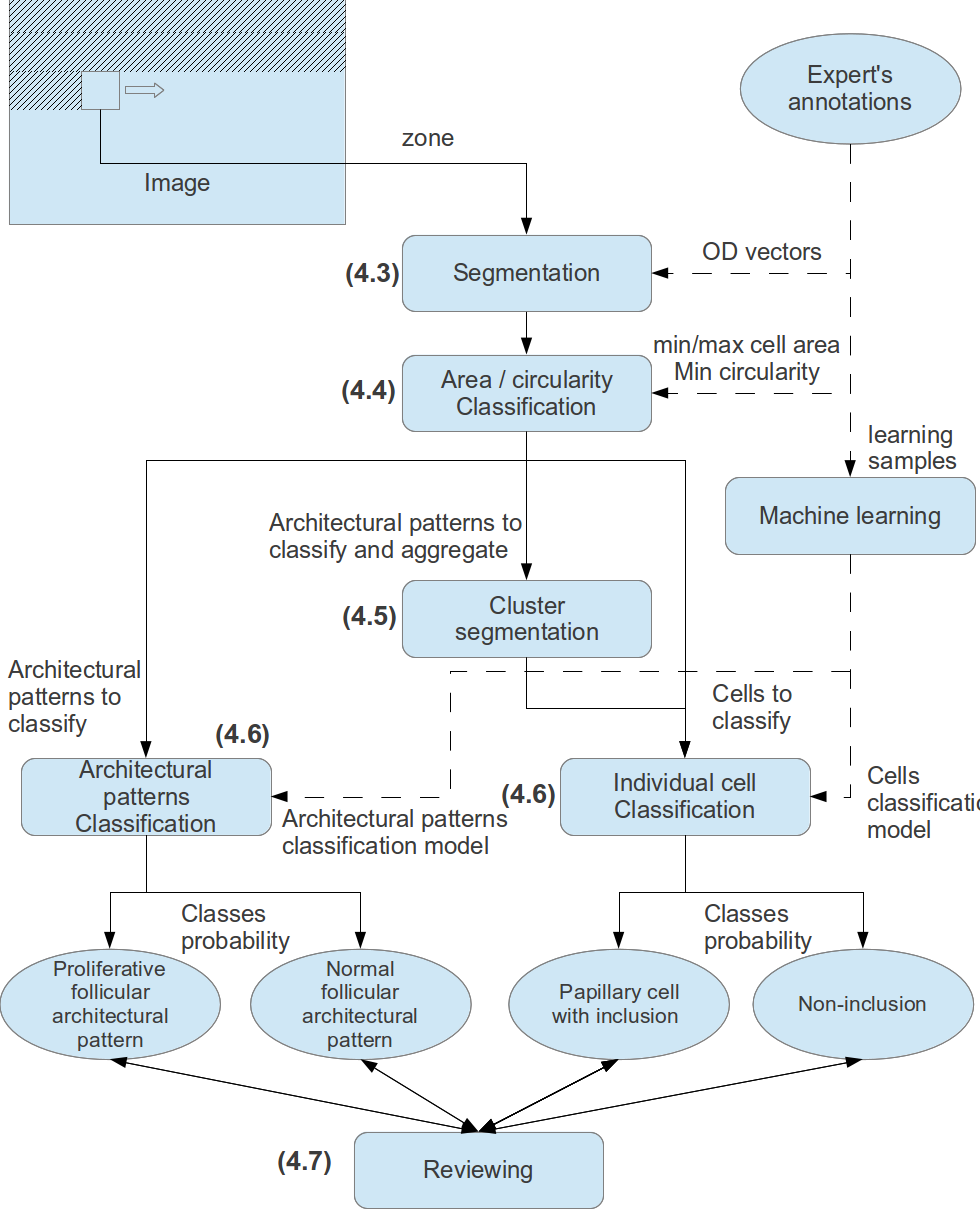
\includegraphics[scale=0.95]{image/adeblire_workflow.png}
	\caption{Antoine Deblire's workflow (source: \cite{adeblire2013})}
	\label{fig:workflow_adeblire}
\end{figure}

\subsection{Segmentation procedures}
The first segmentation procedure was designed for processing the whole slide and relies on a process called color deconvolution \cite{ruifrok2001quantification}. This process consists in retrieving the tissues stains concentration from the RGB image. It appears that cells and patterns have a high concentration of a certain stain in the project images. Therefore, a first segmentation mask is generated by thresholding an image of which each pixel contains an integer value representing the stain concentration for the same pixel in the original image. Some morphological operations are then applied in order to remove noise and fill unwanted holes. Some example segmentations are provided in Figure \ref{fig:first_seg_examples}. It seems that the procedure is able to detect most of the objects of interest although it sometimes fails at covering the whole object area. For instance in the third example image, there is a hole in the mask inside the pattern and this hole covers some cells that should be included in the mask. On the fourth example, one can see three standalone objects above the central pattern. Those objects' masks are smaller than their corresponding cells.

\begin{figure}
	\center
	\subfigure{
		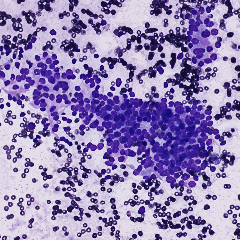
\includegraphics[scale=0.5]{image/slide_segmentation_0_in.png}
		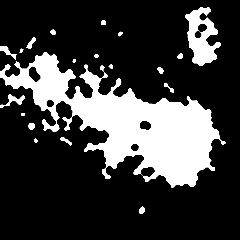
\includegraphics[scale=0.5]{image/slide_segmentation_0_out.png}
		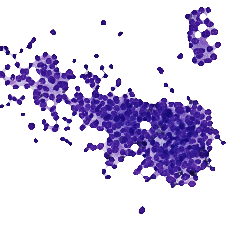
\includegraphics[scale=0.5]{image/slide_segmentation_0_masked.png}
	} \\
	\subfigure{
		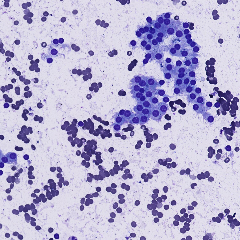
\includegraphics[scale=0.5]{image/slide_segmentation_1_in.png}
		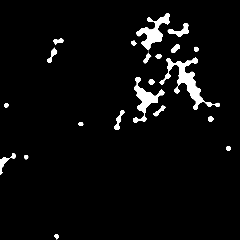
\includegraphics[scale=0.5]{image/slide_segmentation_1_out.png}
		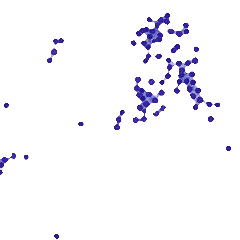
\includegraphics[scale=0.5]{image/slide_segmentation_1_masked.png}
	} \\
	\subfigure{
		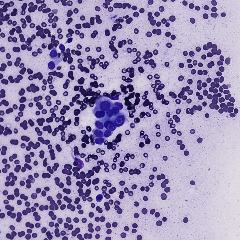
\includegraphics[scale=0.5]{image/slide_segmentation_2_in.png}
		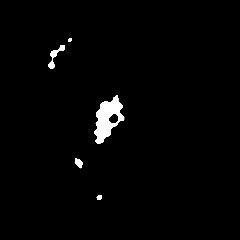
\includegraphics[scale=0.5]{image/slide_segmentation_2_out.png}
		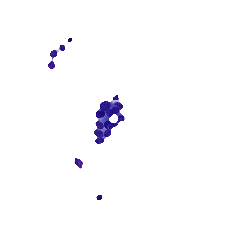
\includegraphics[scale=0.5]{image/slide_segmentation_2_masked.png}
	} \\
	\subfigure{
		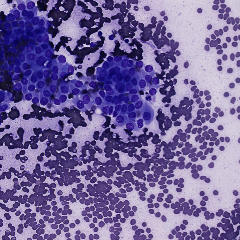
\includegraphics[scale=0.5]{image/slide_segmentation_3_in.png}
		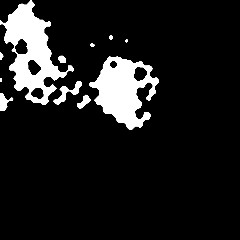
\includegraphics[scale=0.5]{image/slide_segmentation_3_out.png}
		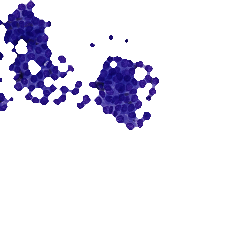
\includegraphics[scale=0.5]{image/slide_segmentation_3_masked.png}
	}
	\caption{First segmentation - examples}
	\label{fig:first_seg_examples}
\end{figure}

The second segmentation procedure is applied to the architectural patterns and was designed to isolate individual cells inside those patterns. The implementation is a little more complicated than the first. Similarly, it starts with a color deconvolution to highlight the cells. However, the stain concentration image is not transformed into a binary mask using a fixed threshold but using Otsu's method. Using the \texttt{findContour} procedure of the OpenCV library as well as morphological operations, independent cells are located and cleaned one after the other. Finally, a watershed algorithm is applied to separate cells that intersects. Some example segmentations are provided in Figure \ref{fig:first_seg_examples}. The segmentation seems to work relatively well on "clean" patterns, that is where cells doesn't overlap much and are clearly distinguishable from the pattern background (see the first two examples in Figure \ref{fig:first_seg_examples}). One "dirty" patterns however, the segmentation performs poorly as it either returns large patches which doesn't correspond to cells or fails to separate overlapping cells.  

\begin{figure}
	\center
	\subfigure{
		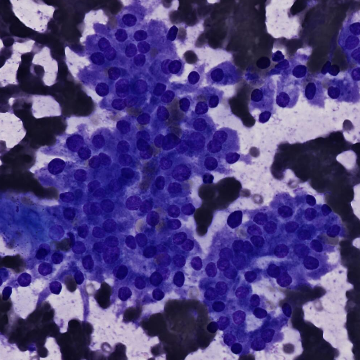
\includegraphics[scale=0.33]{image/aggr_segment_12_in.png}
		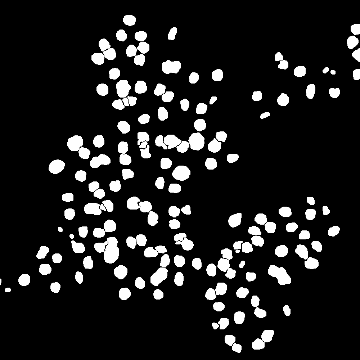
\includegraphics[scale=0.33]{image/aggr_segment_12_out.png}
		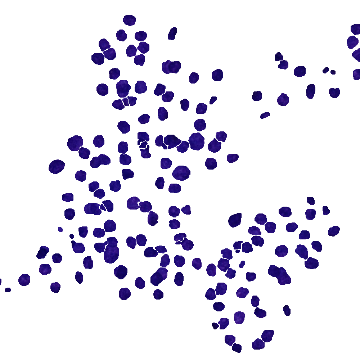
\includegraphics[scale=0.33]{image/aggr_segment_12_masked.png}
	} \\
	\subfigure{
		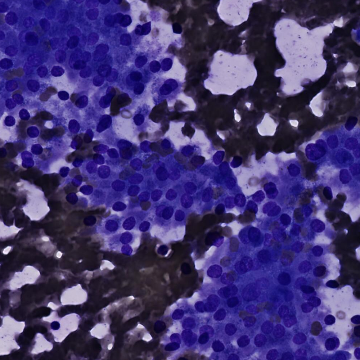
\includegraphics[scale=0.33]{image/aggr_segment_2_in.png}
		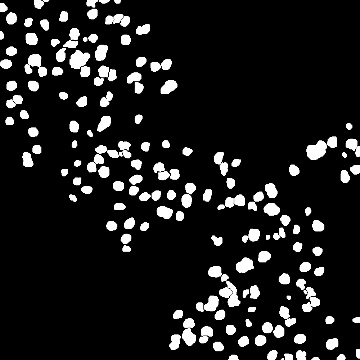
\includegraphics[scale=0.33]{image/aggr_segment_2_out.png}
		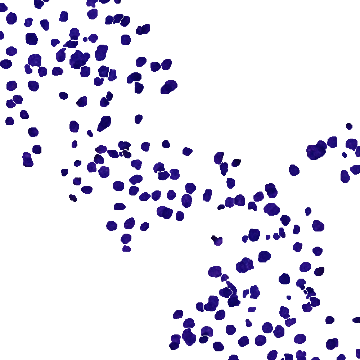
\includegraphics[scale=0.33]{image/aggr_segment_2_masked.png}
	} \\
	\subfigure{
		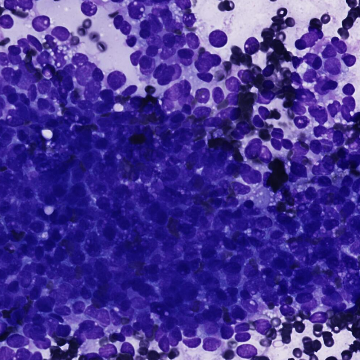
\includegraphics[scale=0.33]{image/aggr_segment_5_in.png}
		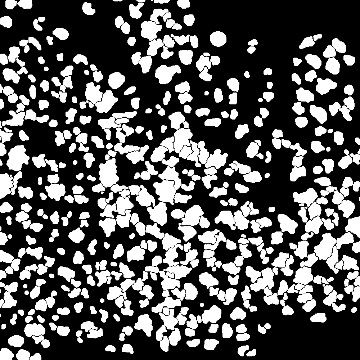
\includegraphics[scale=0.33]{image/aggr_segment_5_out.png}
		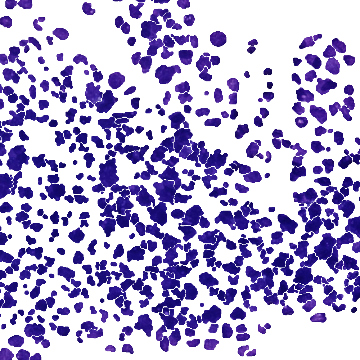
\includegraphics[scale=0.33]{image/aggr_segment_5_masked.png}
	} \\
	\subfigure{
		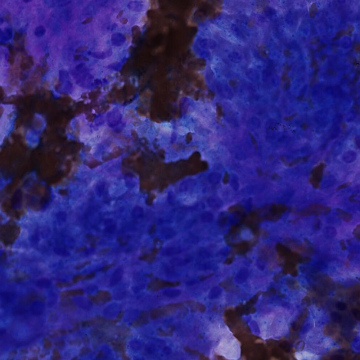
\includegraphics[scale=0.33]{image/aggr_segment_7_in.png}
		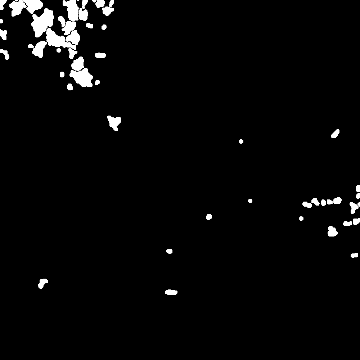
\includegraphics[scale=0.33]{image/aggr_segment_7_out.png}
		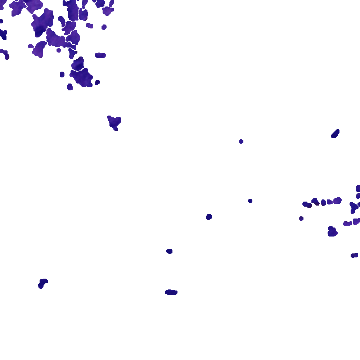
\includegraphics[scale=0.33]{image/aggr_segment_7_masked.png}
	}
	\caption{Second segmentation - examples}
	\label{fig:second_seg_examples}
\end{figure}

While the presented segmentation procedures exhibit some flaws, they were considered acceptable to test the \textit{SLDC} framework.

\subsection{Dispatching procedure}
\label{ssec:thyroid_ad_dispatch}
The step (4.4) consists in dispatching detected objects into four categories: artefacts, cells, clusters and patterns. The categories \textit{artefact} and \textit{cluster} respectively correspond to irrelevant objects and to groups of cells that contains too few of them to be patterns. Even if the author distinguishes patterns and clusters at the dispatching step, objects of both categories are treated equally in the subsequent steps of the algorithm. That is, they are first evaluated by the pattern classifier (for assessing whether they are proliferative or not) and they then are re-segmented. The dispatching is based on four parameters, the cell minimum and maximum areas (respectively, $A_{min}$ and $A_{max}$), the cell minimum circularity $C_{min}$ and the minimum number of cells per pattern $N_{min}$. The values of those parameters are given in Table \ref{tab:adeb_disp_rules}. 

Given $A$ the area of the object of interest, the dispatching rules can be summarized as follows:

\begin{itemize}
	\item \textbf{Artifact}: every object having an area less than $A_{min}$ or and area less than $A_{max}$ and a circularity less then $C_{min}$
	\item \textbf{Cell}: every object having an area such that $A_{min} < A < A_{max}$ and a circularity greater than $C_{min}$
	\item \textbf{Clusters}: every object of which the area is greater than $A_{max}$ and such that it contains at most $N_{min}$ cells:
	\[
		A_{max} < A < N_{min} \times A_{max}
	\]
	\item \textbf{Patterns}: all objects which don't match one of the rule above are considered patterns
\end{itemize}

\begin{table}
	\center
	\begin{tabular}{|c|c|}
		\hline
		$A_{min}$ & 31 $\mu m^2$\\
		\hline
		$A_{max}$ & 102 $\mu m^2$\\
		\hline
		$C_{min}$ & 0.7 \\
		\hline
		$N_{min}$ & 4\\
		\hline
	\end{tabular}
	\caption{Dispatching parameters presented in \cite{adeblire2013}}
	\label{tab:adeb_disp_rules}
\end{table}

The author fixed the dispatching parameters values based on the areas and circularities of experts' annotations. As explained in Section \ref{sec:thyroid_impl_issue}, using those annotations to perform such a task might not be an good idea. Especially, the computed minimum and maximum areas might be a greater than the actual minimum and maximum areas of cells. 

In order the assess whether the dispatching rules are effective for distinguishing cells from patterns, the expert annotations present on Cytomine were used. While those annotations shouldn't be used for setting the parameters, their usage for assessing the method is acceptable. Indeed, in this case, only a qualitative analysis is performed. 

The histograms given in Figures \ref{fig:hist_area_cell_vs_pattern} and \ref{fig:hist_circ_cell_vs_pattern} respectively show the area and circularity distributions of the experts' annotations. First, it appears that, whatever the metric, there is a substantial overlapping between the cells' and patterns' distributions. This has a major consequence for the dispatching procedure presented above. Indeed, as it relies on simple thresholdings, it is ineffective at separating the objects because of the overlapping. Another observation is that the parameters given in Table \ref{tab:adeb_disp_rules} are not relevant as most of the cells would be dispatched as patterns with such values. This observation is confirmed with the scatter plot shown in Figure \ref{fig:scatter_area_circ_cell_vs_pattern}. In this plot, only few cells are effectively dispatched as such (see the blue box in the top left corner of the plot), the others being dispatched as patterns. Given those observations, it is clear that the dispatching procedure must be re-worked.

\begin{figure}
	\center
	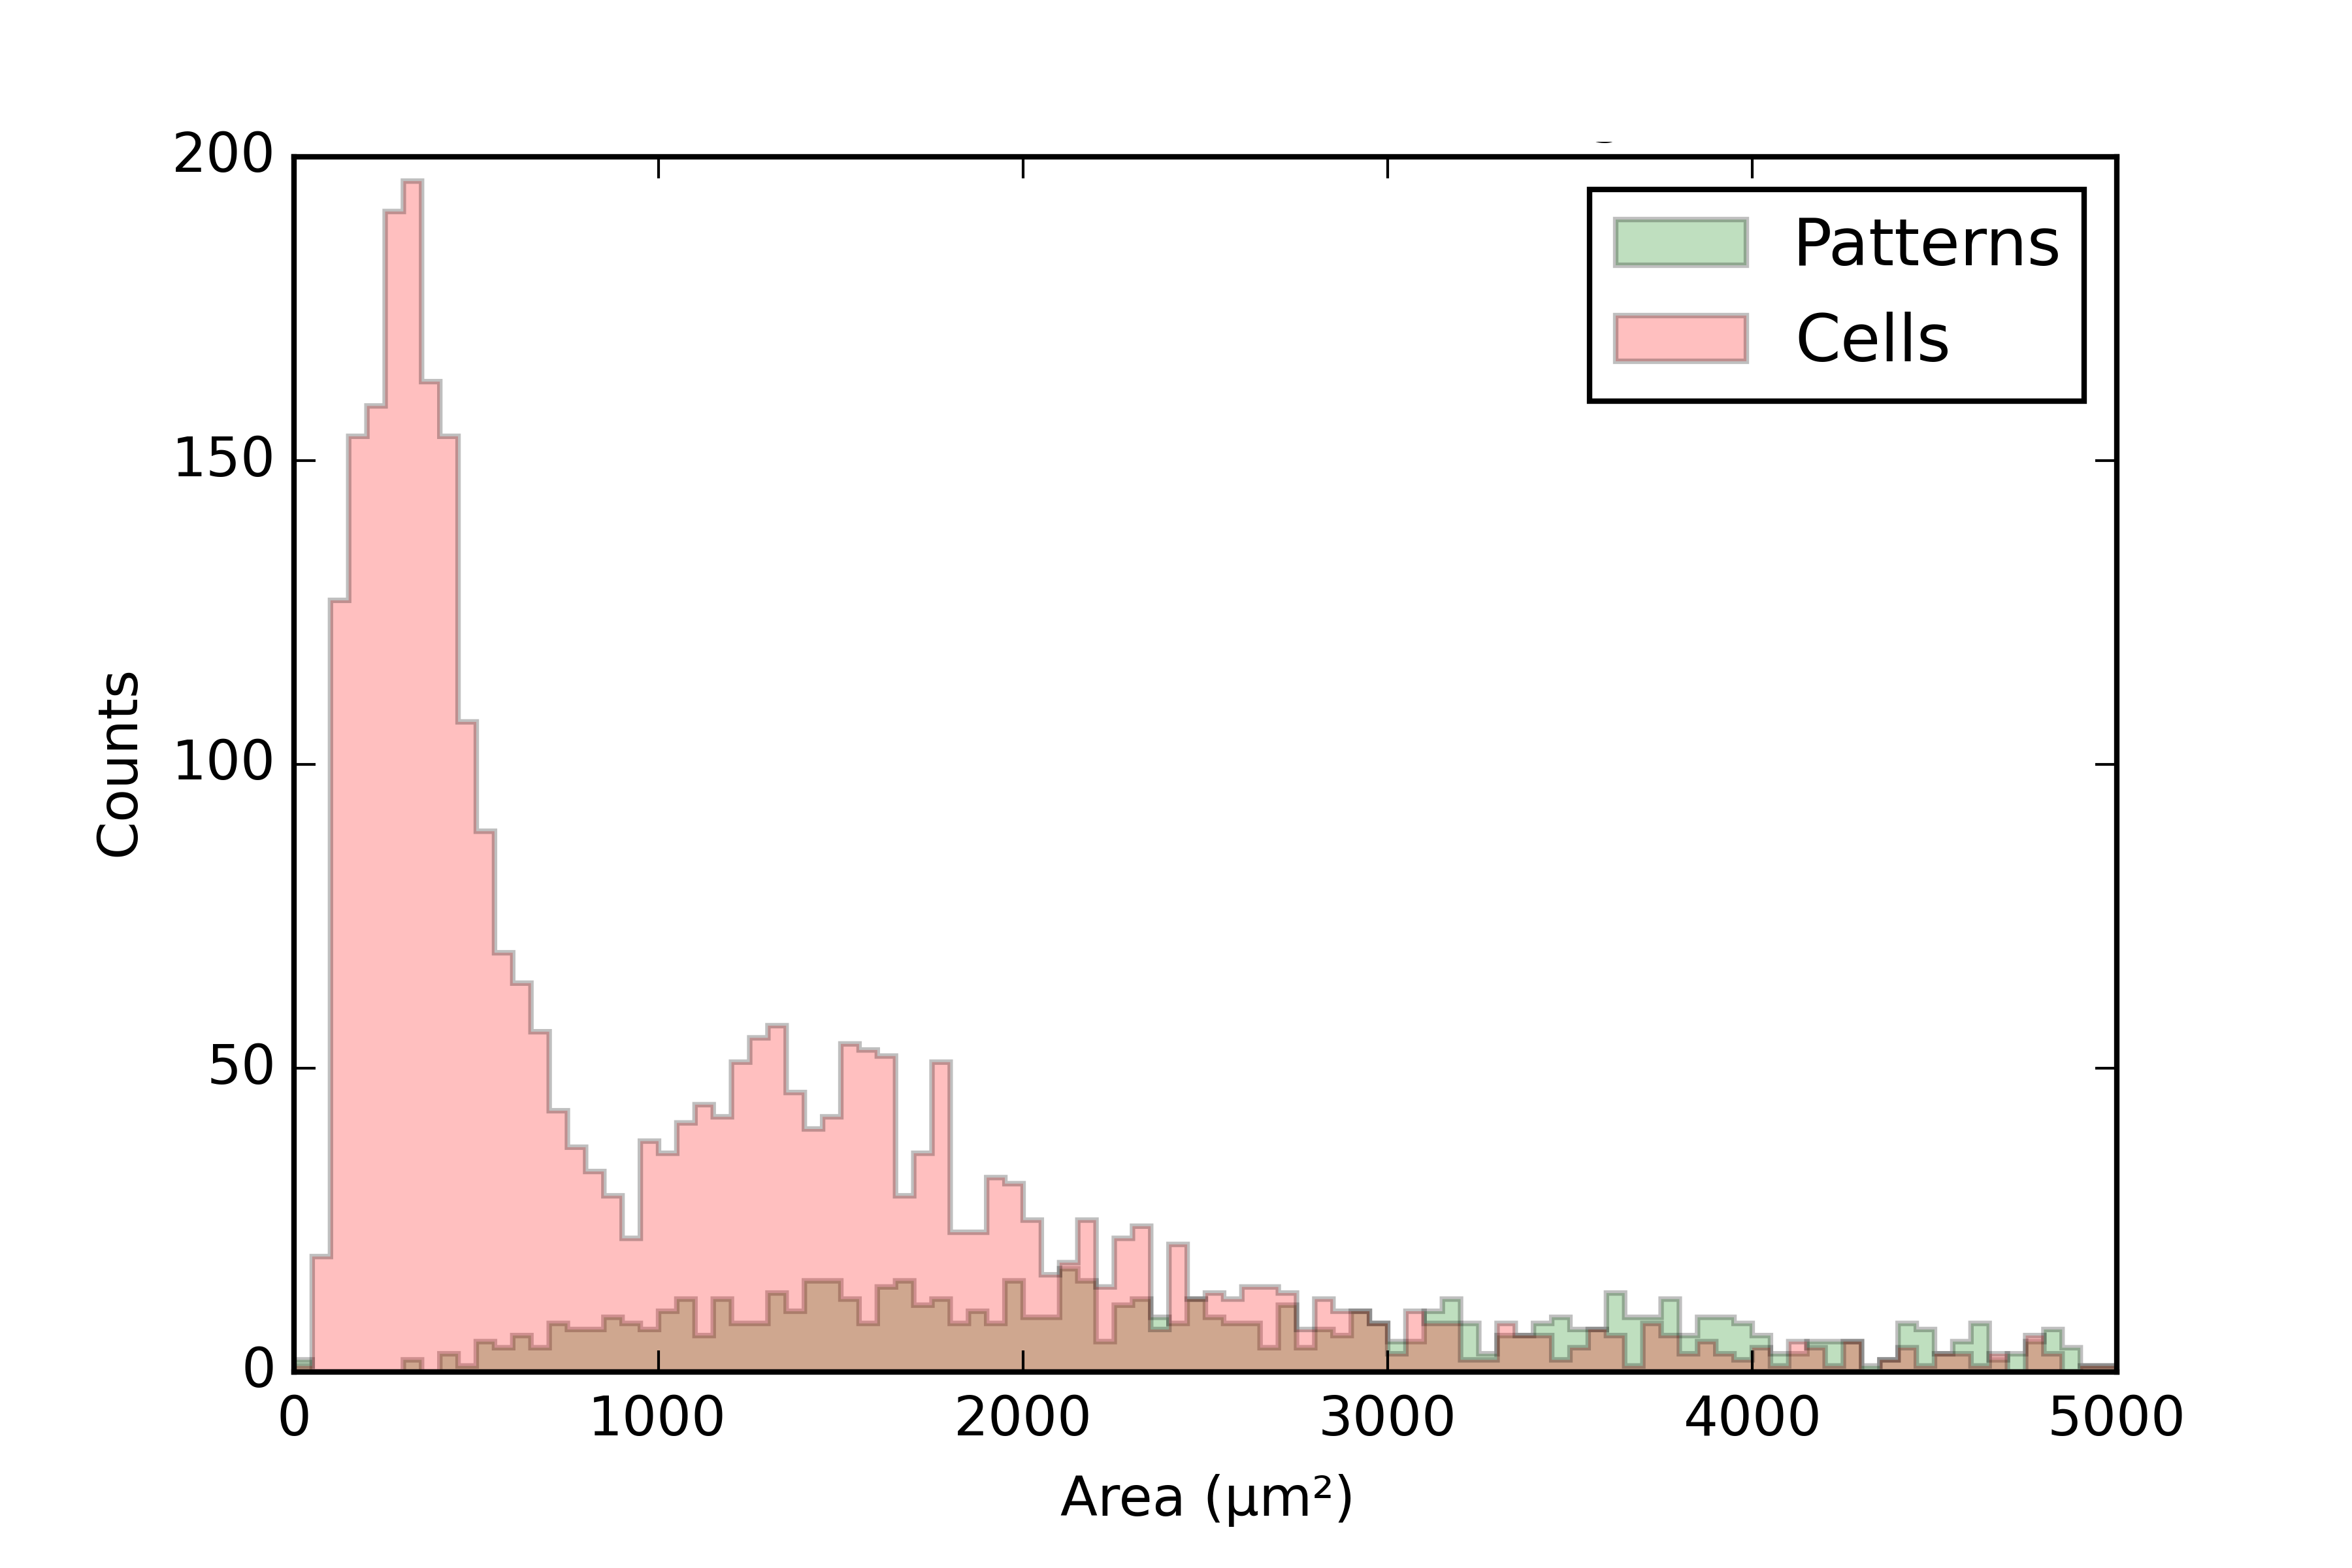
\includegraphics[scale=0.75]{image/cells_patterns_real_area_0_5000.png}
	\caption{Area distributions of the experts' annotations.}
	\label{fig:hist_area_cell_vs_pattern}
\end{figure}

\begin{figure}
	\center
	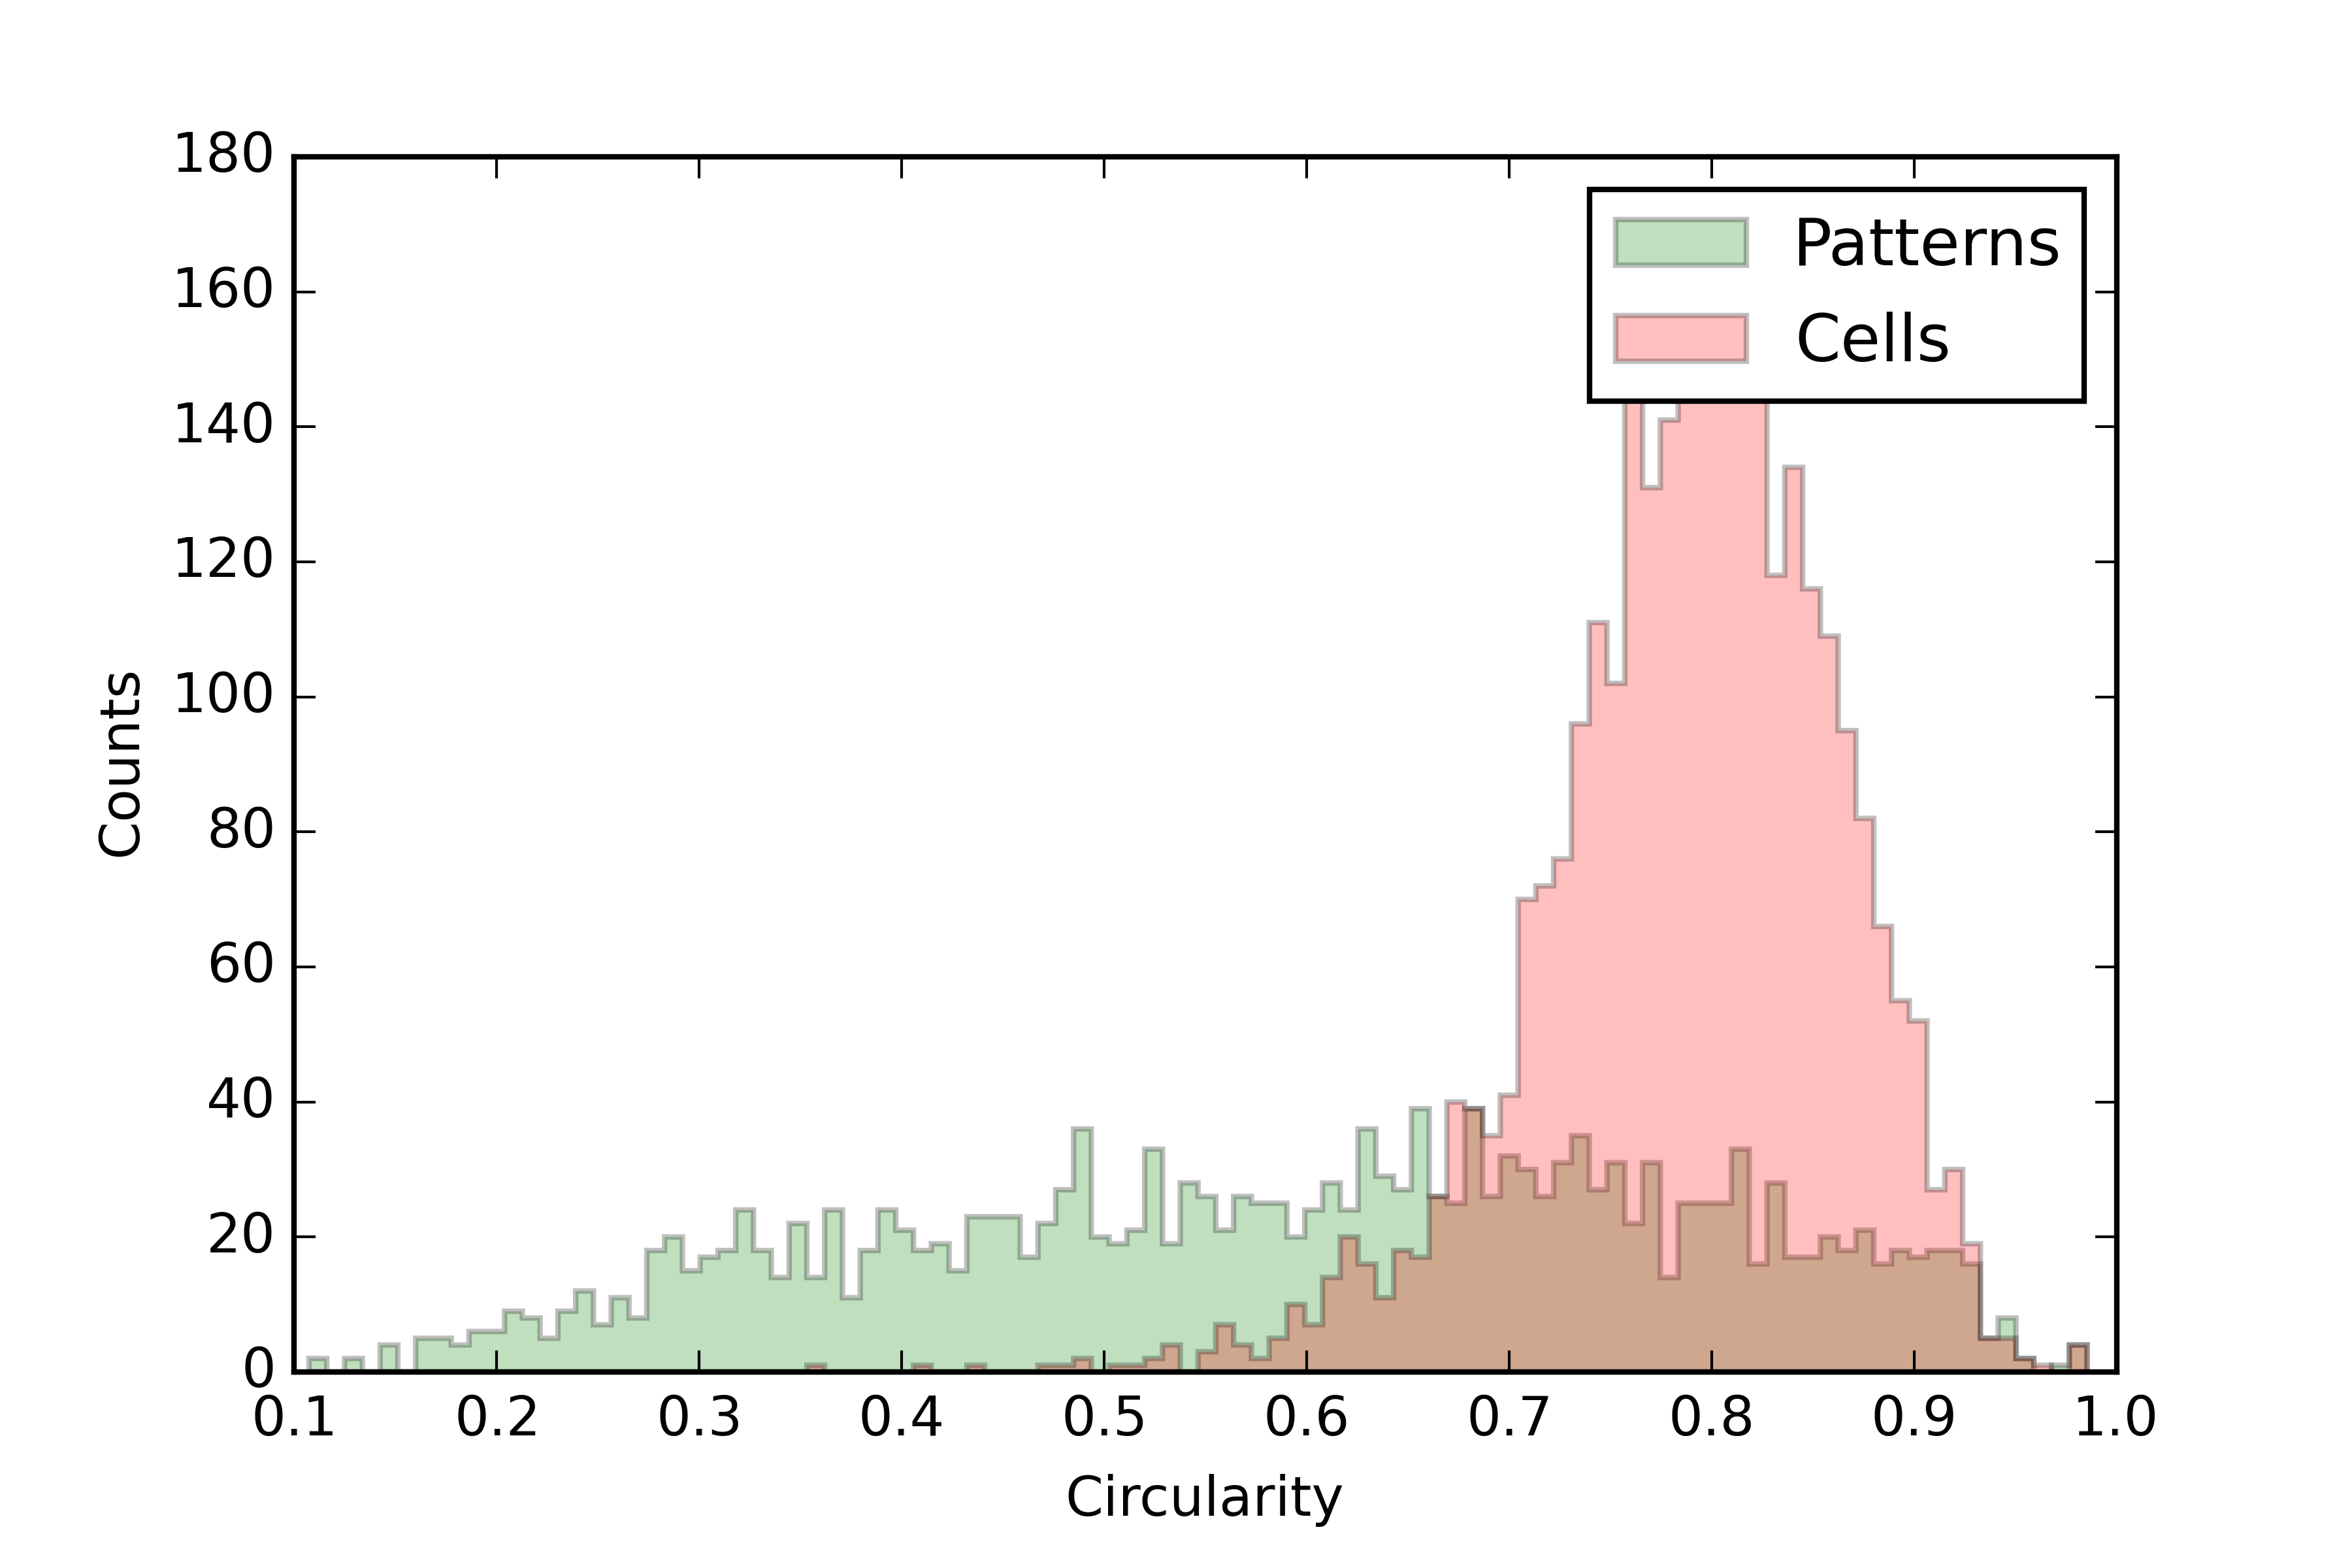
\includegraphics[scale=0.75]{image/cells_patterns_circ.png}
	\caption{Circularity distribution of the experts' annotations.}
	\label{fig:hist_circ_cell_vs_pattern}
\end{figure}


\subsubsection{Improvement}

As relying solely on geometrical properties is not a viable solution, an alternative consists in using the objects' crop image. Especially, the objects' crop would be classified into one of the dispatching categories (i.e. cell, pattern or other) using the random subwindows image classification algorithm \cite{Maree201617} (this algorithm is detailed in Appendix \ref{app:random_subwindows}). A drawback of this solution is that the dimensions of the objects are completely ignored. Given that some patterns might have a similar appearance then cells (color and shape), this might lead to misclassification. 

The overcome the possible problems with the first solution, one could include the geometrical information of the polygons into the learning and prediction processes of the random subwindows algorithm. Especially, the circularity and area would be appended to the feature vector used by the SVM classifier to perform the image classification. This simple operation might not be sufficient however. Indeed, as the features extracted from the ensemble of randomized trees are numerous, the two geometric features would probably not contribute much to the prediction. To overcome this issue, a kernel could be used to increase the contribution of the geometric features. Whereas this solution might yield better results than the first, it requires the experts' annotations of the learning set to be cleaned to avoid the problem mentioned in Section \ref{sec:thyroid_impl_issue}. Moreover, it would require a non-negligible modification of the random subwindows algorithm. It was therefore considered out of the scope of this thesis and the first proposed solution was retained.

\begin{figure}
	\center
	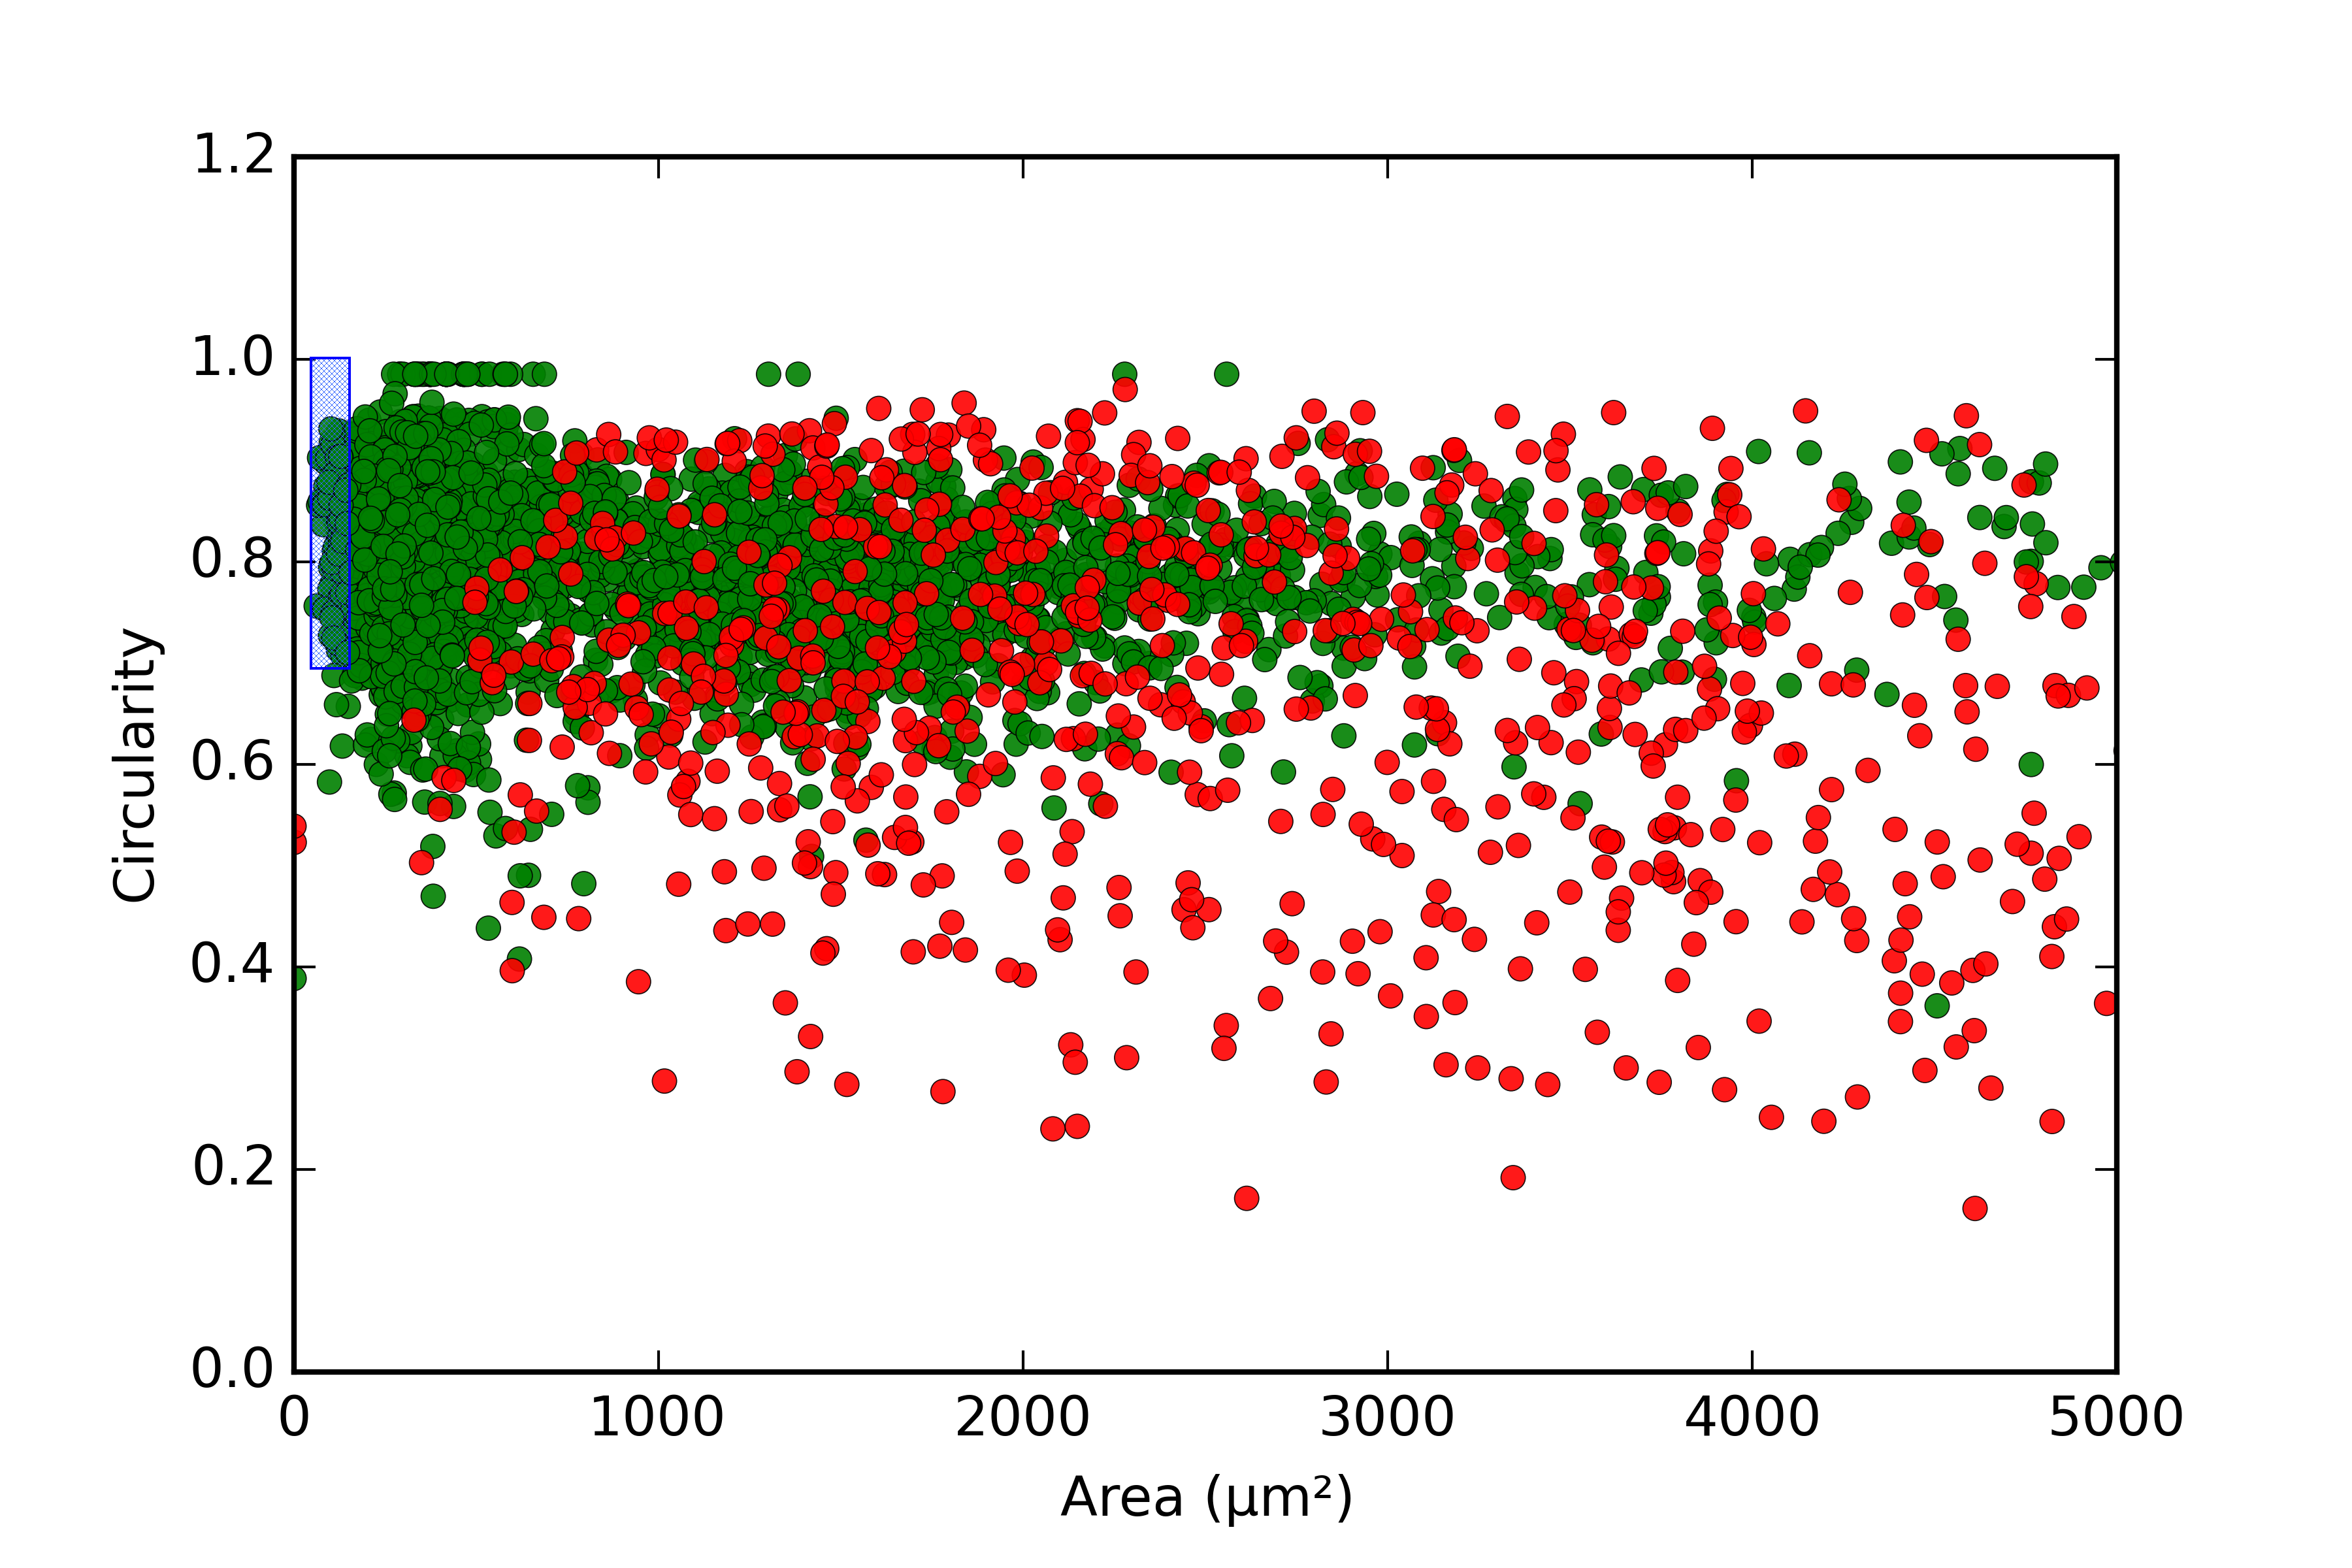
\includegraphics[scale=0.75]{image/scatter_cells_patterns_0_5000.png}
	\caption{Scatter plot, circularity versus area. Green and red dots correspond respectively to cells and patterns. The blue box is the cell dispatching zone.}
	\label{fig:scatter_area_circ_cell_vs_pattern}
\end{figure}

\subsection{Classification}

As soon as objects are dispatched, they have to be classified. In \cite{adeblire2013}, the author uses two classification models: one for cells and another one for patterns. For patterns, a ternary classifier is used and predicts three classes: \textit{proliferative pattern}, \textit{non-proliferative pattern} and \textit{others}. The author states that the third class is needed because with a binary classifier, some objects were classifieed as patterns while they were not. Hopefully, with the new dispatching procedure, those objects will be eliminated before reaching the classifier. It was therefore decided to use a binary classifier for performing this classification. 

As far as the cell classifier is concerned, it predicts two classes: \textit{cells with inclusion} and \textit{non-inclusion}. In addition to the term \textit{cell with inclusion}, the author includes the pseudo inclusions in the positive class. 

The performance study for the various classifiers is given in Section \ref{ssec:thyroid_perf_models}.

\section{Implementation}
\label{sec:thyroid_implementation}
Following the \textit{SLDC} framework philosophy, the problem dependent components have to be defined: an image representation, the segmentation procedures, the dispatching rules and the classifiers. Whenever possible, the components were developed to be reusable for other applications within Cytomine. Those generic components are colored in blue in UML diagrams while the components dependent on the thyroid problem are colored in green.

\subsection{Image representation}

The first component to be defined is the actual representation of the images to be processed, that is, the digitized microscope slides stored on the Cytomine platform. This representation is implemented in the \texttt{CytomineSlide} class which stores an \texttt{ImageInstance}\footnote{The \texttt{ImageInstance} class is defined in the Cytomine Python client} object containing all the information about the slide including its width, height and identifier. To prevent anyone from loading the full image into memory, the implementation of the \texttt{np\_image} raises the \texttt{NotImplementedError} exception. 

In general, when the full image can be loaded into memory the default \texttt{Tile} class can be used. In this case, as this operation is impossible, a class \texttt{CytomineTile} was created to handle the tile image loading. Especially, the call to \texttt{np\_image} triggers an HTTP requests to the Cytomine server to fetch the corresponding image window. If the request fails (e.g. HTTP error) or returns an invalid result (e.g. returned image has an invalid size), a \texttt{TileExtractionError} is raised as advised in the documentation. The class \texttt{CytomineTileBuilder} was created to build \texttt{CytomineTile} objects.

In order to reduce the overall execution time of the workflow, it is essential not to execute two times a same HTTP request for loading the image of a tile. To avoid this, the class \texttt{TileCache} was developed. It implements a simple caching policy using the local file system: when an image window is needed, the \texttt{TileCache} object first checks whether this image was already downloaded. If that is the case, the image can be loaded from the disk. Otherwise, the image is fetched by calling the \texttt{np\_image} method of the underlying tile and stored on the disk before being handed back to the caller. The class also provides methods for adding an alpha mask to the returned image. 

Some additional classes were developed to handle the addition of an alpha mask to an image window (class \texttt{CytomineMaskedWindow}) and to a tile (classes \texttt{CytomineMaskedTile} and \texttt{CytomineMaskedTileBuilder}). This feature is needed for the pattern segmentation procedure which assumes that an alpha mask indicating the position of the pattern is passed with the numpy array. To avoid storing an image representing the alpha mask into the classes, the mask is represented by a polygon. 

The UML diagram of the package containing the image related classes is shown in Figure \ref{fig:uml_cyto_im_repr}.

\begin{figure}
	\center
	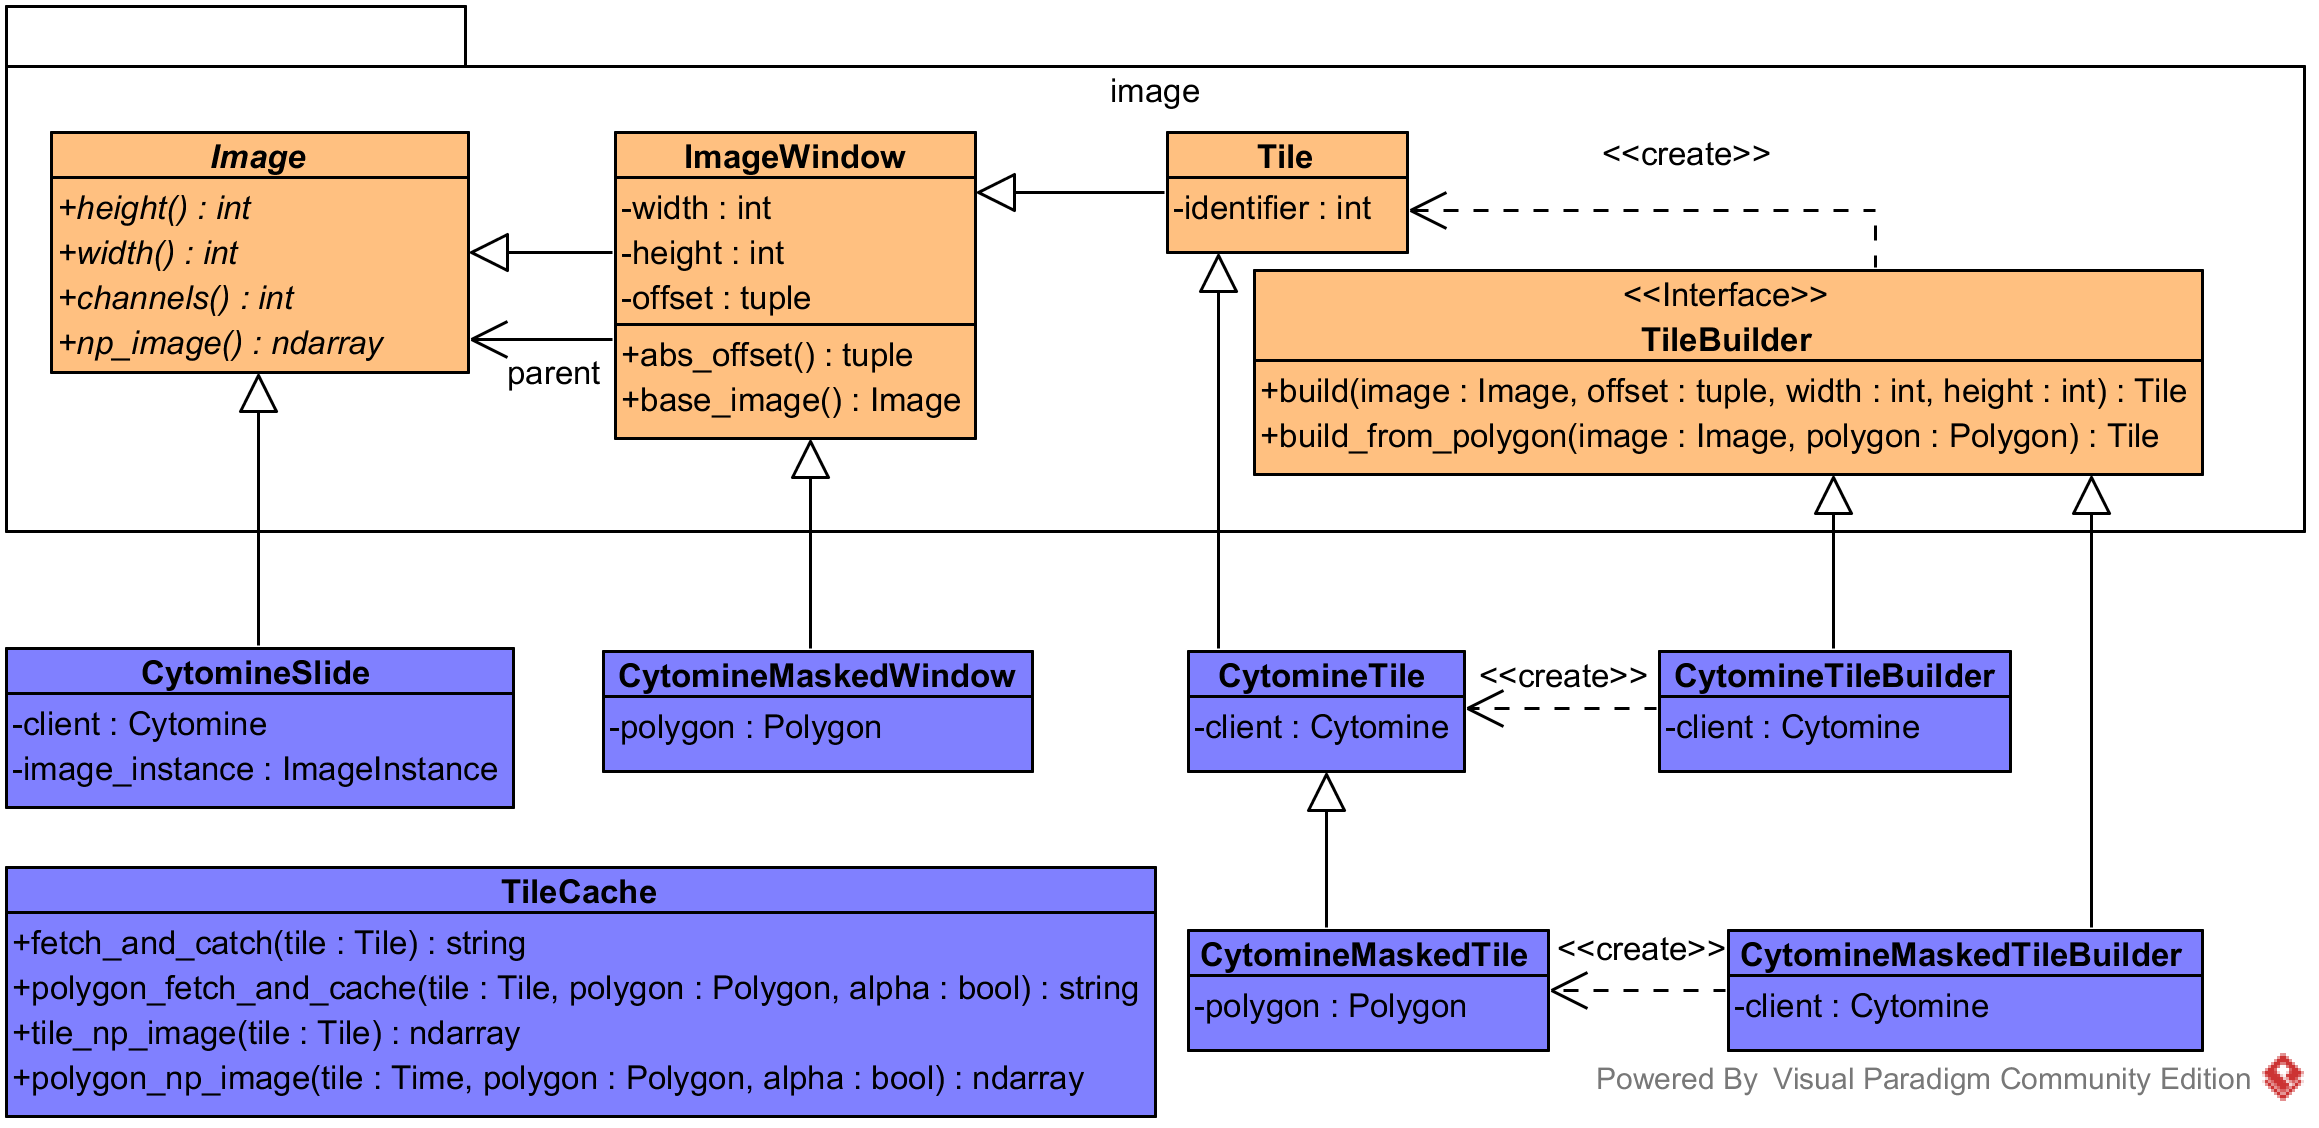
\includegraphics[scale=0.85]{image/thyroid_image.png}
	\caption{UML diagram - Cytomine image representation}
	\label{fig:uml_cyto_im_repr}
\end{figure}

\subsection{Classifier}

All the classification tasks to perform in the context the thyroid problem are performed using the random subwindows algorithm \cite{Maree201617}. Especially, a Python implementation called Pyxit taken from Cytomine \cite{maree2016collaborative} was used. The central class of this implementation is the \texttt{PyxitClassifier} class which provides an scikit-learn-like interface to the algorithm (i.e. the methods \texttt{fit}, \texttt{transform}, \texttt{predict},...). In order to use this class within the framework, a class \texttt{PyxitClassifierAdapter} was developed. The \texttt{predict\_batch} method is implemented as follows.

 First, the crops of the polygons passed to the method are fetched and stored on the disk using a \texttt{TileCache} (thanks to the cache, the HTTP request is only executed the first time the crops are requested). Because there can be a lot of polygons, the fetching of the crops is parallelized and the number of available processes can be specified at the construction of the \texttt{PyxitClassifierAdapater} object. Each available process is passed a set of polygons of which the crops must be fetched in order to reduce the serialization overhead (see Section \ref{sssec:work_parallel}). If some crops cannot be fetched whatever the reason, the corresponding polygons are associated a class \texttt{None} and a probability 0. Moreover the user is notified with the logger about the crops that couldn't be fetched.

As Pyxit works with images stored on the disk, a list containing the filepath of the images to classify is generated and passed to the \texttt{\_predict} method. This method implements the generation of the classification labels and probabilities. If a SVM classifier was provided at construction of the \texttt{PyxitClassifierAdapter} object, then the variant of the random subwindows algorithm that uses the extremely randomized trees as feature learner is used. That is, the Pyxit classifier is used to generate the features that are passed to the SVM classifier for predicting the labels. Otherwise, the variant that uses the extremely randomized trees as direct classifier is used. 

Finally, the \texttt{predict\_batch} method aggregates the results returned by the \texttt{\_predict} method with the fake labels and probabilities generated for the polygons of which the crops couldn't be fetched.

A static method is also provided for constructing a \texttt{PyxitClassifierAdapter} object from a serialized Pyxit model. Especially, the method deserializes the \texttt{PyxitClassifier} object as well as the SVM classifier if one is provided and passe them to the adapter's constructor. This method also sets the number of processes to use for fetching the crops. If the number of available processors is less than five, then all of them are used to fetch the crops. Otherwise, five processors are used. This value was chosen in order to avoid overloading Cytomine server when the number of available processors is high.

The UML diagram of the \texttt{PyxitClassifierAdapter} class is shown in Figure \ref{fig:uml_cyto_classifiers}.

\begin{figure}
	\center
	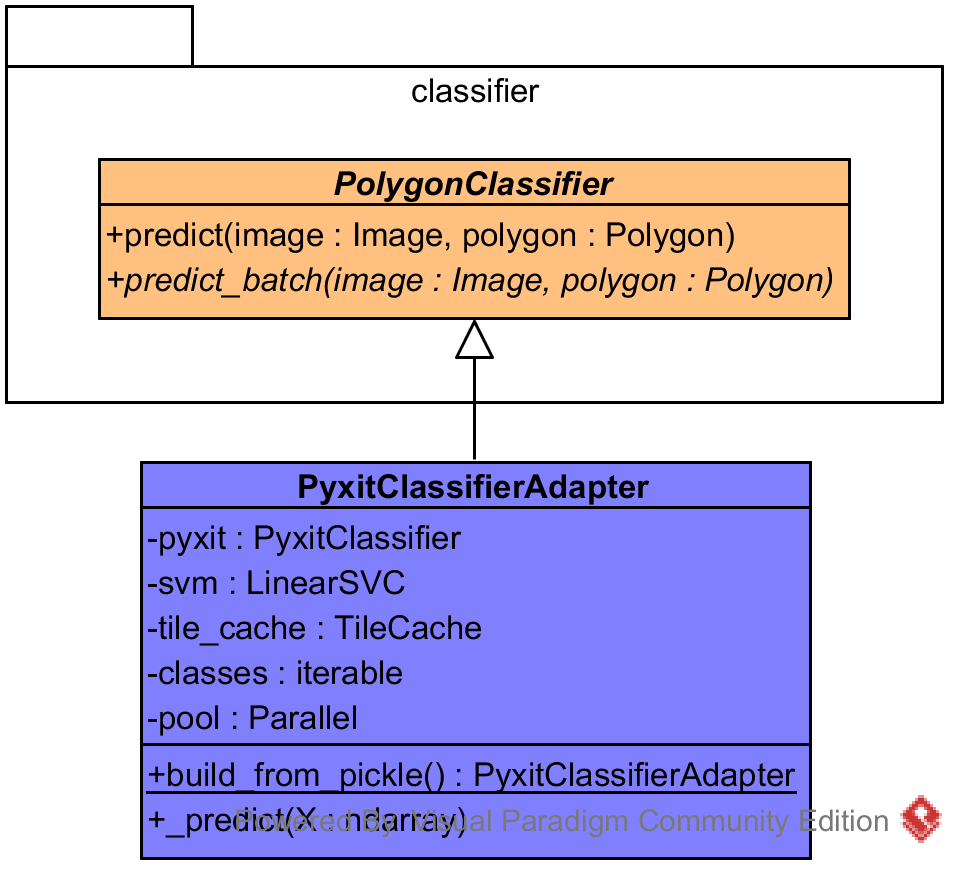
\includegraphics[scale=0.85]{image/thyroid_classifiers.png}
	\caption{UML diagram - Classifier}
	\label{fig:uml_cyto_classifiers}
\end{figure}

\subsection{Dispatching rules}

As explained in Section \ref{ssec:thyroid_ad_dispatch}, the chosen dispatching method relies on a classifier of which the predicted class is the dispatching index. Especially, the classifier was built to predict the label 0 for cells, 1 for patterns and 2 for the other objects.

To take advantage of the features provided by the class \texttt{PyxitClassifierAdapter} (i.e. caching, parallel fetching,...), it was reused and encapsulated in two classes extending \texttt{DispatchingRule}. The implementation of the rules' \texttt{evaluate\_batch} method is therefore straightforward. It first calls the \texttt{predict\_batch} method of the classifier adapter object and then generates a list of boolean values according to the returned classification labels. For the first rule, \texttt{CellRule}, \texttt{True} is associated to polygons of which the returned label is 0. For the second, \texttt{AggregateRule}, \texttt{True} is associated with polygons of which the predicted label is 1.

Unfortunately, this organization implies that the polygons marking patterns and other objects will be classified two times by the same classifier. Indeed, because of the dispatching structure imposed by the framework, the polygons that are not matched by the first rule are evaluated by the second. This could be avoided by refactoring the framework or by implementing another dispatching strategy.

The UML diagram containing the dispatching rule classes is shown in Figure \ref{fig:uml_cyto_disp_rules}.

\begin{figure}
	\center
	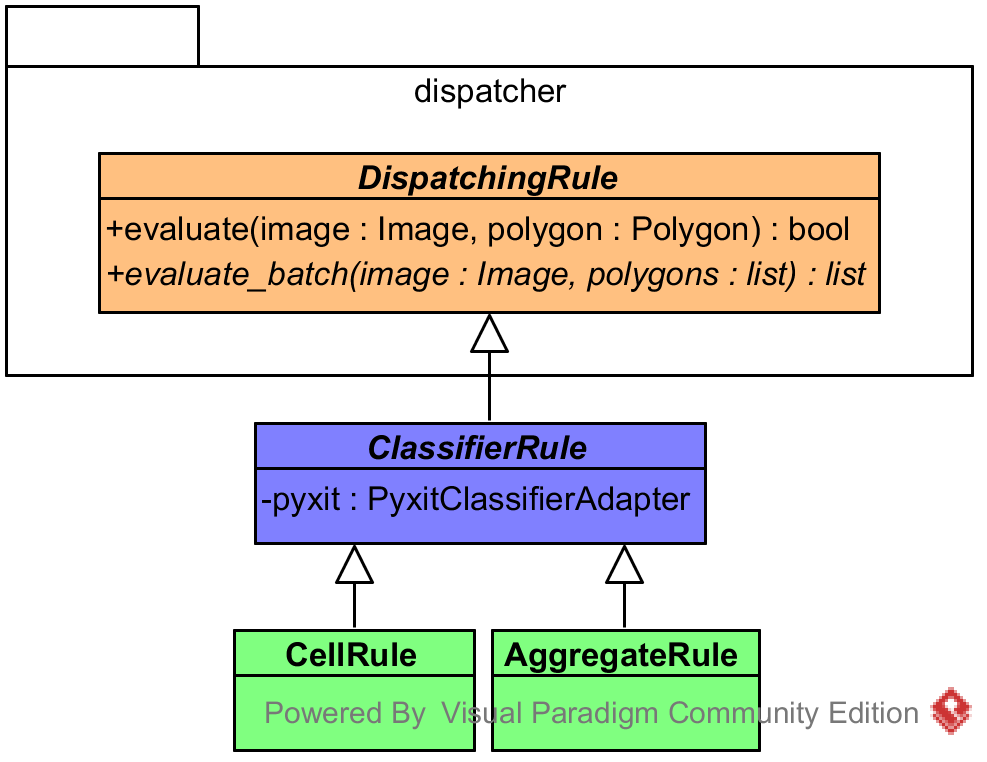
\includegraphics[scale=0.85]{image/thyroid_dispatching_rules.png}
	\caption{UML diagram - Thyroid workflow dispatching rules}
	\label{fig:uml_cyto_disp_rules}
\end{figure}

\subsection{Segmentation}

The segmentation procedures were implemented in two classes, \texttt{SlideSegmenter} and \texttt{AggregateSegmenter}. Both implementation were taken from Antoine Deblire's source code. Whereas the slide segmentation could be used almost directly without modification, the recovered aggregate segmentation procedure didn't work. It was therefore re-implemented following the explanations provided in the master thesis as well as the few comments present in the source code. After few tests, it appeared that both segmentation procedures were really slow because of the color deconvolution. Especially, to execute the color deconvolution on a 4 mega-pixels image yielded more than 2 seconds execution time. A first optimization pass was done over the function in order to reduce its execution time to 1 second (same image dimensions). The UML diagram containing the segmenter classes is shown in Figure \ref{fig:uml_cyto_segmenters}.

\begin{figure}
	\center
	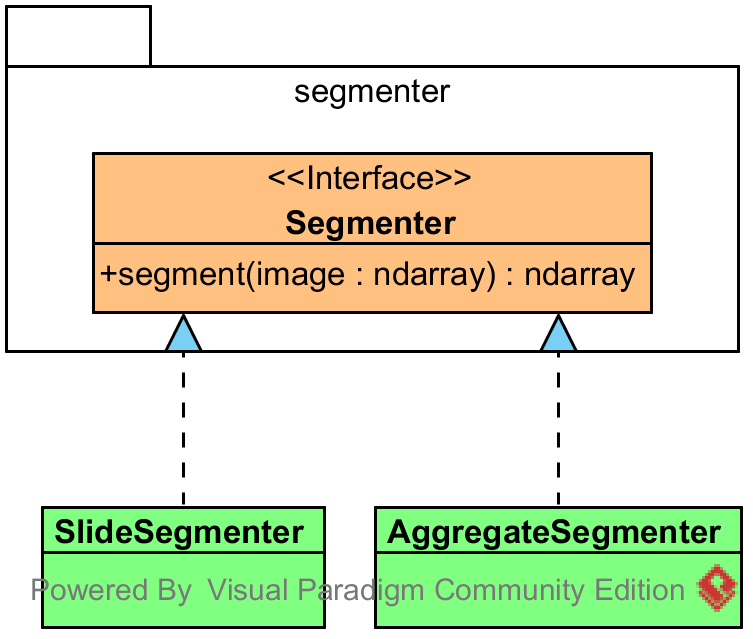
\includegraphics[scale=0.85]{image/thyroid_segmenters.png}
	\caption{UML diagram - Segmenter classes}
	\label{fig:uml_cyto_segmenters}
\end{figure}

\subsection{Chaining}

The chaining package of the framework must be used to define which detected objects (i.e. the patterns) must be re-segmented. First, an image provider must be defined to generate the \texttt{CytomineSlide} to be processed. This logic is implemented in the \texttt{SlideProvider} class. Then, the selection of the objects to be processed by the second workflow must be defined as a \texttt{WorkflowExecutor}. Especially, the class \texttt{AggregateWorkflowExecutor} was implemented to fulfill this role. The class defines the method \texttt{get\_windows} which implements the selection of objects to be re-segmented and the generation of \texttt{CytomineMaskedWindow} objects to be processed by the second workflow. Moreover, it extends the class \texttt{PolygonTranslatorWorkflowExecutor} because the polygons generated by this phase needs to be translated back into the full image reference system. The final component to be defined is the post processor which is passed all the detected objects and their classes. In the context of the thyroid problem, the post processor should upload the generated polygons and classes as annotations on the Cytomine platform. This logic is implemented in the \texttt{post\_process} method of the \texttt{ThyroidPostProcessor} class. Unfortunately, the Cytomine API doesn't provide any request for uploading annotations by batches and each annotation has to be added with two HTTP requests: one for uploading the geometry and another for uploading the predicted class and associated probability. To avoid waiting for each request to terminates before sending another one, the process was parallelized. The UML diagram containing the chaining classes is shown in Figure \ref{fig:uml_cyto_chaining}.


\begin{figure}
	\center
	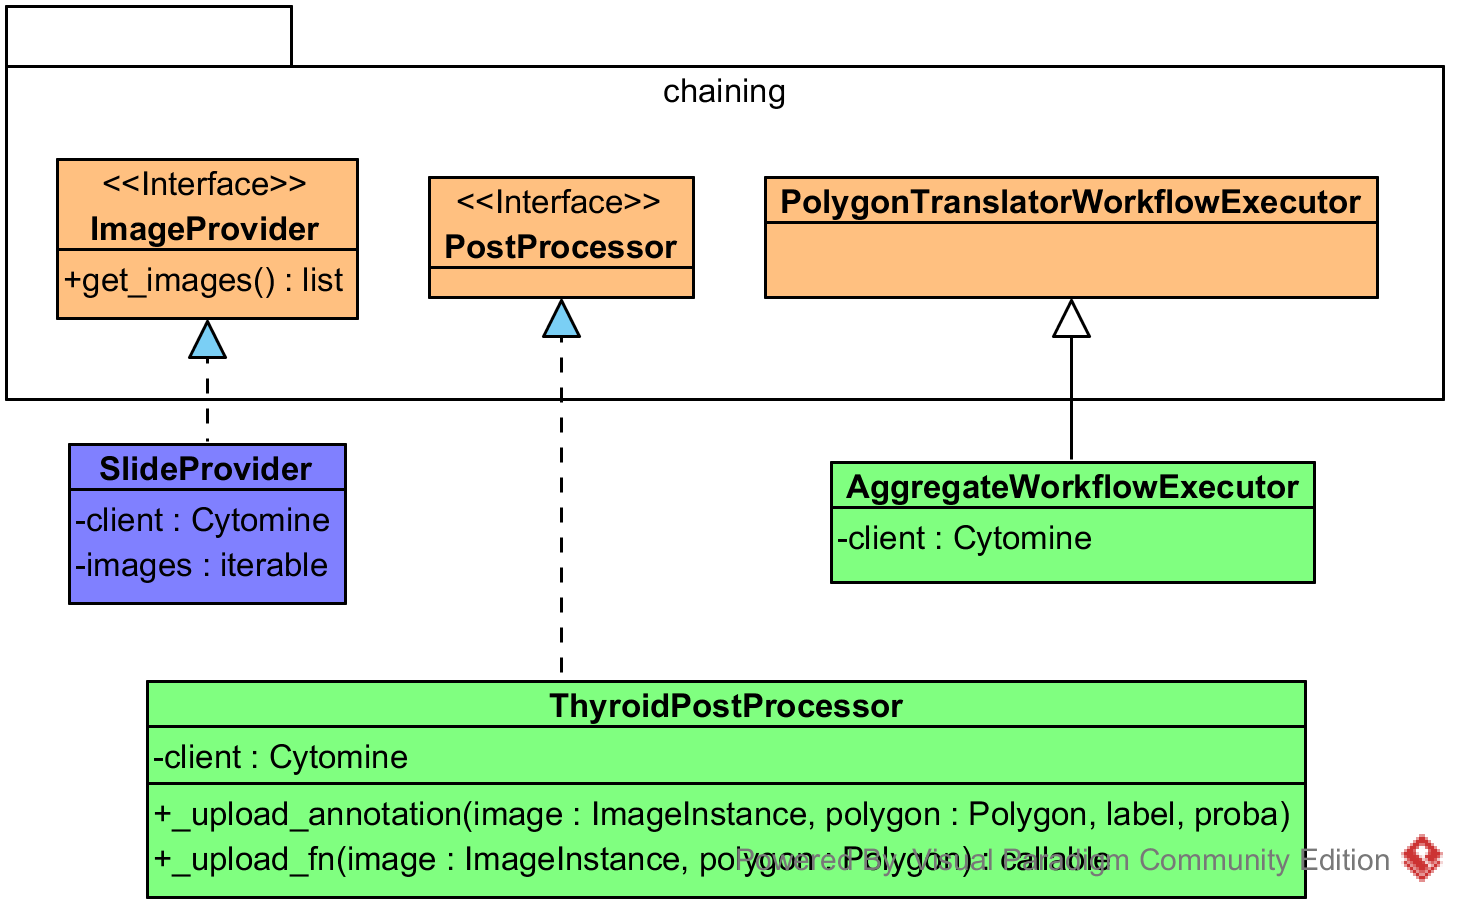
\includegraphics[scale=0.85]{image/thyroid_image_provider.png}
	\caption{UML diagram - Chaining classes}
	\label{fig:uml_cyto_chaining}
\end{figure}


\section{Performance analysis}
\label{sec:thyroid_perf}

\subsection{Classification models}
\label{ssec:thyroid_perf_models}
\subsubsection{Test set and cross validation}
\subsubsection{Dispatching model}
\subsubsection{Pattern classifier}
\subsubsection{Cell classifier}

\subsection{Execution times}

\subsection{Memory}

\subsection{Overall}
	\newpage
	% End chapter 3 : thyroid case ============
	
	% Start conclusion ========================
	\chapter{Conclusion}
	This thesis proposes \textit{SLDC}, a generic framework for object detection and classification in mutli-gigapixel images. 
It provides implementers with a concise way of formulating their algorithm by declaring only problem dependent-components: segmentation procedures and classification models. Behind the scenes, the framework takes care of problem-independent concerns. For instance, in order to avoid loading the full image into memory, it splits this image in tiles which are processed independently. Parallelism is also encapsulated by the framework which applies it to accelerate tiles processing. Are also provided: a powerful and customizable logging system informing the user about errors and overall progress, a way of executing several workflows one after another on a same image and robustness so that errors of which the impact is negligible does not stop the whole program. The framework is available on GitHub as a Python library. 

The framework was then applied to a real-world problem, thyroid nodule malignancy diagnosis, in order to assess its performances. Especially, a workflow developed for this problem in a previous master thesis was analysed, improved and re-implemented using the framework. 

The results are promising: the effective execution time of the workflow was less than 10 minutes on a 8 gigapixels image (executed on 32 processes). This time is mostly due to design choice linked to the implementation and the framework only induces a negligible overhead. Some improvements can be done both at the framework and workflow levels. Especially, some other operations of the former could be parallelized and the current parallelization could be optimized.

As far as the thyroid case is concerned, the developed workflow does not provide a production-ready solution yet because it sometimes fails at detecting objects of interest and produces an important number of false positives. However, the analysis provided in this thesis already points out elements which needs to be improved (segmentation procedures, classification models,...) providing a baseline for any further development on this case.

	% End conclusion ==========================
	
	\appendix
	
	% Start tile topology appendix ============
	\chapter{Tile topology}
	\label{apdx:tile_topology}

As presented in Section \ref{sssec:work_image_repr}, the tile topology objects associate unique increasing identifiers to tiles. Using this representation allows to reach a $\mathcal{O}(1)$ time complexity for all the methods of the class \texttt{TileTopology}. Indeed, the results produced by those methods can be computed using simple formulas. In the following formulas, $i$ refers to a tile identifier:

\begin{itemize}
	\item The number $t_{row}$ of tiles on a row is given by:
	\begin{equation} \label{eqn:nb_tile_on_row}
		t_{row} = \left\{
		\begin{array}{cl}
			\left\lceil \dfrac{w - o_p}{w_m - o_p}\right\rceil&\text{, if } w > w_m\\
			1&\text{, otherwise}\\
		\end{array}
		\right.	
	\end{equation}
	\item The number $t_{col}$ of tiles on a column is given by Equation \ref{eqn:nb_tile_on_row} applied to the image height $h$ and maximum tile height $h_m$ instead of $w$ and $w_m$. 
	\item The total number $t$ of tiles in the tile topology is simply $t_{row} \times t_{col}$.
	\item The neighbour tiles identifiers can be obtained by performing subtractions and additions. For instance, for a tile  which is not on the edge of the image, the identifiers of its left, top, right and bottom neighbours are respectively $i - 1$, $i - t_{row}$, $i + 1$, $i + t_{row}$.
	\item The tile offset $(t_{\text{off},x}, t_{\text{off},y})$ can be retrieved as follows:
	\begin{eqnarray}
		t_{\text{off},x} = (t_{row} - o_p) \times \left[(i-1) \mod t_{row} \right] \\
		t_{\text{off},y} = (t_{col} - o_p) \times \left\lfloor\frac{i - 1}{t_{row}}\right\rfloor
	\end{eqnarray} 
\end{itemize}
	\newpage
	% End tile topology appendix ==============
	
    % Start ontology ==========================
	\chapter{Ontology}
	\label{app:ontology}
The ontology associated with the Thyroid project on Cytomine is the following:

\begin{enumerate}
	\item Architectural patterns:
	\begin{itemize}
		\item Normal follicular architectural pattern
		\item Proliferative follicular architectural pattern
		\item Proliferative follicular architectural pattern (minor sign)
	\end{itemize}
	\item Nuclear features:
	\begin{itemize}
		\item Papillary cell NOS
		\item Normal follicular cells
		\item Normal follicular cell with pseudo-inclusion (artefact)
		\item Papillary cell with ground glass nuclei
		\item Papillary cell with nuclear grooves
		\item Papillary cell with inclusion
	\end{itemize}
	\item Others:
	\begin{itemize}
		\item Macrophages
		\item Red blood cells
		\item PN (polynuclear)
		\item Colloid
		\item Artefacts
		\item Background
	\end{itemize}
\end{enumerate}

% TODO add images
	\newpage
	% End ontology ============================
	
	% Start Pyxit =============================
	\chapter{ET-FL and ET-DIC image classifiers}
	\label{app:random_subwindows}
Random subwindows \cite{Maree201617} is an image classification algorithm. The first step of the algorithm consists in transforming the $N$ input images. This is done by extracting a set of $N_w$ random subwindows from each image. A random subwindow is a square patch of random size extracted at a random position in an image. The extracted windows are then resized to a fixed size patch $(w, h)$. Those transformation operations generates a dataset containing $N\times N_w$ objects and $w \times h$ attributes. 

The second step consists in passing this dataset to a classifier which will actually predict the image's classification label from those subwindows. In \cite{Maree201617}, two classification methods are proposed.

The first uses extremely randomized trees \cite{Geurts2006} as direct classifier: that is, each window is predicted a label and the full image label is determined by a majority vote over the predicted classes of this image's windows.

The second variant uses extremely randomized trees as feature learner rather than a direct classifier and relies on a SVM classifier to produce the prediction. 
In this variant each image is represented as a vector of which the dimensionality equals the number of terminal nodes in the ensemble of randomized trees and where the $i^{th}$ feature is the number of windows that reached the $i^{th}$ leaf node of the forest divided by the total number of windows. This vector is then passed to the SVM classifier to predict the image classification label.




	\newpage
	% End Pyxit ===============================
	
	% Start Cross validation ==================
	\chapter{Cross validation}
	Cross validation
	\newpage
	% End Cross validation ====================
	
	% Start Performance table =================
	\chapter{Execution times}
	\label{app:exec_times}
In Tables \ref{tab:perf_time_size_and_jobs}, ..., are given detailed execution times for executions of the workflow on several images. All execution times are given in seconds. More details about the fields of those tables are given hereafter:

\begin{enumerate}
	\item \textbf{Run information}: global information about the run
	\begin{itemize}
		\item \textit{Run number}: a number associated with the execution in order to ease referencing those runs in the thesis
		\item \textit{Image width and height}: width and height (in pixels) of the image processed by the run
		\item \textit{Tile width and height}: width and height (in pixels) of the tiles used by the tile topology to break down the images in smaller chunks
		\item \textit{Tiles}: number of tiles containing in the topology
		\item \textit{Jobs}: number of processed assigned to the execution
		\item \textit{RAM}: maximum amount of memory available for the run to execute
	\end{itemize}
	\item \textbf{Polygons}: information about the polygons found by the run
	\begin{itemize}
		\item \textit{Found}: number of polygons found across all tiles 
		\item \textit{Merged}: number of polygons resulting from the merging phase
		\item \textit{Cell}: number of polygons dispatched to the cell classifier
		\item \textit{Pattern}: number of polygons dispatched to the pattern classifier
		\item \textit{Dispatched}: total number of dispatched polygons
	\end{itemize}
	\item \textbf{L-S-L}: execution times of the \textbf{L}oad-\textbf{S}egment-\textbf{L}ocate phase. This phase is parallelized.
	\begin{itemize}
		\item \textit{Loading}: total amount of time for loading tiles into memory (on separate processes)
		\item \textit{Segment}: total amount of time for segmenting the tiles (on separate processes)
		\item \textit{Location}: total amount of time for locating polygons in segmented tiles (on separate processes)
		\item \textit{Overall}: actual amount of time for processing all the tiles (wall-clock time)
	\end{itemize}
	\item \textbf{Dispatching}: execution times of the dispatching phase
	\begin{itemize}
		\item \textit{Cell model}: variant of the random subwindows algorithm used for dispatching polygons
		\item \textit{Fetch 1}: times needed for fetching the crops of the polygons to dispatch from the Cytomine server
		\item \textit{Cells}: amount of time needed for finding whether the polygons should be dispatched to the cell classifier or not
		\item \textit{Fetch 2}: time needed for fetching the crops of the polygons to dispatch to the pattern classifier. Normally, it should always be small as all the crops have already been downloaded and cached by the\textit{Fetch 1} step
		\item \textit{Patterns}: amount of time for finding whether the polygons should be dispatched to the pattern classifier or not
		\item \textit{Overall}: total amount of time for dispatching the polygons 
	\end{itemize}
	\item \textbf{Classification}: execution times of the classification phase
	\begin{itemize}
		\item \textit{Fetch 3}: times needed for fetching the crops of the polygons to be processed by the cell classifier. As for \textit{Fetch 2}, those times should be low. 
		\item \textit{Cells}: amount of time for classifying the cells 
		\item \textit{Fetch 4}: times needed for fetching the crops of the polygons to be processed by the cell classifier. As for \textit{Fetch 2}, those times should be low.
		\item \textit{Patterns}: amount of time for classifying patterns
		\item \textit{Overall}: total amount of time for classifying the dispatched polygons
	\end{itemize}
	\item \textbf{Net.}: for \textit{Network}, time spent for sending network requests and waiting for responses
	\begin{itemize}
		\item \textit{Caching}: amount of time needed for fetching and caching the tiles of the topology
		\item \textit{Upload}: amount of time needed for uploading the dispatched polygons to the Cytomine server
	\end{itemize}
	\item \textbf{Total}: 
	\begin{itemize}
		\item \textit{Not net. 1}: total execution time of the run from which was deduced the \textit{Caching} and \textit{Upload} execution times. 
		\item \textit{Not net. 2}: total execution time of the run from which was deduced the \textit{Caching}, \textit{Upload}, \textit{Fetch 1}, \textit{Fetch 2}, \textit{Fetch 3} and \textit{Fetch 4} execution times
		\item \textit{Overall}: total execution time of the run. Might not equal the sum of the various steps executions times. Indeed, some operations performed between those steps are not included in the corresponding execution times
	\end{itemize}		
	
\end{enumerate}

\begin{table}
	\footnotesize
	\center
	\begin{tabular}{|c|c|c|c|c|c|c|c|}
		\hline
		\parbox[t]{2mm}{\multirow{9}{*}{\rotatebox[origin=c]{90}{Run information}}} & Run nb. & 1 & 2 & 3 & 4 & 5 & 6 \\
		& Image & 728725 & 728725 & 728725 & 728725 & 728725 & 728725 \\
		& Width & 131072 & 131072 & 131072 & 131072 & 131072 & 131072 \\
		& Height & 57856 & 57856 & 57856 & 57856 & 57856 & 57856 \\
		& Tile width & 512 & 512 & 512 & 1024 & 1024 & 1024 \\
		& Tile height & 512 & 512 & 512 & 1024 & 1024 & 1024 \\
		& Tiles & 29900 & 29900 & 29900 & 7353 & 7353 & 7353 \\
		& Jobs & 16 & 32 & 64 & 16 & 32 & 64 \\
		& RAM (Go) & 100 & 100 & 100 & 100 & 100 & 100 \\
		&  &  &  &  &  &  & \\
		\parbox[t]{2mm}{\multirow{5}{*}{\rotatebox[origin=c]{90}{Polygons}}} & Found & 10009 & 10009 & 10009 & 8418 & 8418 & 8418 \\
		& Merged & 7294 & 7294 & 7294 & 7195 & 7195 & 7195 \\
		& Cell & 5172 & 5169 & 5169 & 5141 & 5118 & 5128 \\
		& Pattern & 1581 & 1567 & 1572 & 1528 & 1540 & 1554 \\
		& Dispatched & 6753 & 6736 & 6741 & 6669 & 6658 & 6682 \\
		&  &  &  &  &  &  & \\
		\parbox[t]{2mm}{\multirow{4}{*}{\rotatebox[origin=c]{90}{LSL}}} & Loading & 593.145 & 1544.394 & 773.857 & 537.775 & 951.596 & 1210.165 \\
		& Segment & 4801.758 & 6736.784 & 7321.667 & 5148.477 & 7376.851 & 7757.463 \\
		& Location & 2083.925 & 2492.705 & 2472.753 & 2033.105 & 2427.312 & 2690.361 \\		
		& \textbf{Overall} & \textbf{476.952} & \textbf{348.405} & \textbf{199.245} & \textbf{536.385} & \textbf{351.635} & \textbf{206.755} \\
		&  &  &  &  &  &  & \\
		& Merging & 14.324 & 14.451 & 18.086 & 40.640 & 40.605 & 40.774 \\
		&  &  &  &  &  &  & \\
		\parbox[t]{2mm}{\multirow{6}{*}{\rotatebox[origin=c]{90}{Dispatching}}} & Model & ET-FL & ET-FL & ET-FL & ET-FL & ET-FL & ET-FL \\
		& Fetch 1 & 251.098 & 5.148 & 1.678 & 108.064 & 5.766 & 1.485 \\
		& Cells & 765.858 & 758.031 & 739.323 & 762.242 & 758.993 & 741.434 \\
		& Fetch 2 & 0.750 & 1.079 & 0.959 & 1.077 & 0.860 & 0.830 \\
		& Patterns & 112.861 & 140.930 & 135.782 & 142.667 & 141.502 & 137.354 \\
		& \textbf{Overall} & \textbf{1130.706} & \textbf{905.329} & \textbf{877.897} & \textbf{1014.201} & \textbf{907.267} & \textbf{881.252} \\
		&  &  &  &  &  &  & \\
		\parbox[t]{2mm}{\multirow{7}{*}{\rotatebox[origin=c]{90}{Classification}}} & Model & ET-DIC & ET-DIC & ET-DIC & ET-DIC & ET-DIC & ET-DIC \\
		& Fetch 3 & 1.372 & 1.602 & 1.664 & 1.200 & 1.431 & 1.167 \\
		& Cells & 19.248 & 14.213 & 12.614 & 20.849 & 14.141 & 12.165 \\
		& Model & ET-DIC & ET-DIC & ET-DIC & ET-DIC & ET-DIC & ET-DIC \\
		& Fetch 4 & 0.667 & 0.729 & 0.851 & 0.582 & 0.781 & 0.623 \\
		& Patterns & 7.527 & 5.639 & 4.978 & 7.465 & 5.212 & 5.136 \\
		& \textbf{Overall} & \textbf{28.865} & \textbf{22.240} & \textbf{20.162} & \textbf{30.149} & \textbf{21.622} & \textbf{19.149} \\
		&  &  &  &  &  &  & \\
		\parbox[t]{2mm}{\multirow{2}{*}{\rotatebox[origin=c]{90}{Net.}}} & Caching & 6193.270 & 27.953 & 4.178 & 3858.679 & 10.786 & 4.255 \\
		& Upload & 4993.832 & 444.564 & 444.000 & 4039.734 & 471.113 & 435.173 \\
		&  &  &  &  &  &  & \\
		\parbox[t]{2mm}{\multirow{3}{*}{\rotatebox[origin=c]{90}{Total}}} & Not net. 1 & 1652.464 & 1291.571 & 1116.922 & 1621.971 & 1321.591 & 1148.385 \\
		& Not net. 2 & 6646.296 & 1736.134 & 1560.921 & 5661.706 & 1792.703 & 1583.558 \\
		& \textbf{Overall} & \textbf{12839.566} & \textbf{1764.088} & \textbf{1565.100} & \textbf{9520.385} & \textbf{1803.489} & \textbf{1587.814} \\
		\hline
	\end{tabular}
	\caption{Effects of varying the tile sizes and the available number processes on the execution times. Test image (728725) has dimensions $728725 \times 131072$.}
	\label{tab:perf_time_size_and_jobs}
\end{table}

\begin{table}
	\footnotesize
	\center 
	\begin{tabular}{|c|c|c|c|c|c|c|c|}
		\hline
		\parbox[t]{2mm}{\multirow{8}{*}{\rotatebox[origin=c]{90}{Run information}}} & Run nb. & 1 & 2 & 3 & 4 & 5 & 6 \\
		\cline{2-8}		
		& Image & 716528 & 728725 & 728725 & 728725 & 8120444 & 8120444\\
		& Width & 163840 & 131072 & 131072 & 131072 & 172032 & 172032\\
		& Height & 95744 & 57856 & 57856 & 57856 & 104704 & 104704\\
		& Tile width & 512 & 1024 & 1024 & 512 & 1024 & 1024\\
		& Tile height & 512 & 1024 & 1024 & 512 & 1024 & 1024\\
		& Tiles & 61750 & 7353 & 7353 & 29900 & 17510 & 17510\\
		& Jobs & 16 & 16 & 16 & 16 & 100 & 100\\
		& RAM {\tiny(Go)} & 32 & 32 & 32 & 100 & 1000 & 1000\\
		&  &  &  &  &  &  & \\ 
		\parbox[t]{2mm}{\multirow{5}{*}{\rotatebox[origin=c]{90}{Polygons}}} & Found & 49442 & 8385 & 8385 & 9998 & 201974 & 202853\\
		& Merged & 42573 & 7164 & 7164 & 7330 & 183782 & 183992\\
		& Cell & 81 & 149 & 2468 & 2755 & / & 109510\\
		& Pattern & 2384 & 833 & 1077 & 1393 & / & 28960\\
		& Dispatched & 2465 & 982 & 3545 & 4148 & 174389 & 138470\\
		&  &  &  &  &  &  & \\
		\parbox[t]{2mm}{\multirow{4}{*}{\rotatebox[origin=c]{90}{LSL}}} & Loading & 129001.7494 & 53514.2437 & 53710.7671 & 20688.7785 & 247867.2302 & 247462.9641\\
		& Segment & 9485.1414 & 4743.8858 & 4719.1849 & 6713.7414 & 10068.0100 & 9896.3807\\
		& Location & 4209.0709 & 1971.8888 & 1961.1859 & 2738.4343 & 4458.5427 & 4471.3817\\
		& \textbf{Overall} & \textbf{9158.3703} & \textbf{3829.1936} & \textbf{3835.3665} & \textbf{1930.2026} & \textbf{2686.0573} & 2724.0464\\
		&  &  &  &  &  &  &  \\
		& Merging & 91.0140 & 57.6108 & 57.7504 & 36.0167 & 2052.1225 & 1972.3464\\
		&  &  &  &  &  &  &  \\
		\parbox[t]{2mm}{\multirow{6}{*}{\rotatebox[origin=c]{90}{Dispatching}}} & Model & ET-FL (r.) & ET-FL & ET-FL & ET-FL & ET-FL & ET-DIC\\
		& Fetch 1 & 313.2474 & 146.9693 & 102.1281 & 234.7505 & 19962.1771 & 8697.8838\\
		& Cells  & 288.3571 & 92.5044 & 493.3059 & 607.5096 & 56615.5098 & 381.4897\\
		& Fetch 2 & 1.2727 & 0.4469 & 0.6815 & 1.0183 & 124.6983 & 153.0141\\
		& Patterns & 279.2642 & 73.3186 & 156.8081 & 153.6380 & 348.1110 & 155.1389\\
		& \textbf{Overall} & \textbf{883.0553} & \textbf{313.4013} & \textbf{753.0886} & \textbf{997.1051} & \textbf{81731.1864} & \textbf{9391.5655}\\
		&  &  &  &  &  &  &  \\
		\parbox[t]{2mm}{\multirow{5}{*}{\rotatebox[origin=c]{90}{Classification}}} & Fetch 3 & 0.5211 & 0.2369 & 0.6788 & 1.0994 & 124.6983 & 20.2389\\
		& Cells & 1.0911 & 1.1579 & 10.7008 & 12.6491 & 277.9153 & 235.6081\\
		& Fetch 4 & 0.9426 & 0.4519 & 0.4557 & 1.0570 & 348.1110 & 145.5594\\
		& Patterns & 13.2939 & 6.3793 & 7.2864 & 10.1172 & 37.3042 & 50.3971\\
		& \textbf{Overall} & \textbf{15.8702} & \textbf{8.2355} & \textbf{19.1502} & \textbf{24.9634} & \textbf{811.8941} & \textbf{452.8960}\\
		&  &  &  &  &  &  &  \\
		& Upload & 5661.45 & 290.23 & 2431.7649 & 345.5561 & 28151.8883 & 8588.6074 \\
		\hline
	\end{tabular}
	\caption{Cytomine server}
	\label{tab:execution_times}
\end{table}
	\newpage
	% End Performance table ===================
	
	% Start list of figures ===================
	%\chapter*{Notations}
	%\begin{tabular}{lcl}
	\multicolumn{3}{l}{\textbf{Image :}} \\ 
	& $\mathcal{I}$ & An image \\
	& $w$ & The width of an image \\
	& $h$ & The height of an image \\
	& $c$ & The number of channels of an image \\
	& $\mathcal{I}_{hw}$ & An two dimensional image of width $w$ and height $h$ \\	
	& $p_{ij}$ & A pixel at row $i$ and column $j$ of a two dimensional image \\
	& $\mathcal{B}$ & A binary image \\
	& $b_{ij} \in \{0, 1\}$ & A pixel of a binary image\\
	& $P$ & A polygon \\
	\multicolumn{3}{l}{\textbf{Machine learning :}} \\ 
	& $T(\cdot)$ & A classifier \\
	& $C$ & A classification label \\
\end{tabular}
	%\newpage
	% End list of figures =====================


	% Start list of tables ====================
	\listoftables
	% End list of tables ======================
	
	% Start list of figures ===================
	\listoffigures
	% End list of figures =====================
	
	% Start bibliography ======================
	\printbibliography[heading=bibintoc]
	% End bibliography ========================
\end{document}
